\documentclass[sigconf]{acmart}
\usepackage{setspace}
\usepackage{caption}
\usepackage{amsmath,amsfonts,bm,amsthm}
\usepackage[linesnumbered,ruled]{algorithm2e}
\usepackage{graphicx}
\usepackage[tight,normal]{subfigure}
\usepackage{multirow,makecell,url,footmisc}
\usepackage{enumerate}
\usepackage{lineno}
%\usepackage[left]{lineno}
\usepackage{textcomp}
\usepackage{booktabs} % For formal tables
\usepackage{mathtools}
\usepackage{threeparttable}
%\usepackage{epstopdf}
\usepackage[american]{babel}
% \usepackage[numbers]{natbib}
\usepackage{color}
\usepackage{appendix}
\usepackage{comment}
\usepackage{blindtext}
\newcommand{\argmax}{\mathop{\arg\max}}
\newcommand{\argmin}{\mathop{\arg\min}}
\newcommand{\med}{\mathop{\textrm{med}}}
\newcommand{\x}{{\bf x}}
\newcommand{\w}{{\bf w}}
\newcommand{\z}{{\bf z}}
\newcommand{\y}{{\bf y}}
\newcommand{\X}{\mathcal{X}}
\newcommand{\Y}{\mathcal{Y}}
\newcommand{\expect}{\mathbb{E}}
\newcommand{\Var}{\mathrm{Var}}
\newcommand{\sign}{\mathtt{sign}}
\newcommand{\mathI}{\mathcal{I}}
\newcommand{\defeq}{\stackrel{\text{def}}{=}}
\newcommand{\EDIT}{\color{red}}
\newcommand{\bs}{\boldsymbol}

\newcommand{\chuhao}{\fontsize{1.25pt}{\baselineskip}\selectfont}

%\DeclareMathOperator*{\argmax}{argmax}

\fancyhead{}
\settopmatter{printacmref=false}
\renewcommand\footnotetextcopyrightpermission[1]{}
\pagestyle{plain}
%\settopmatter{printcopyright=false}
\copyrightyear{2018} 
\acmYear{2018} 
\setcopyright{acmcopyright}
\acmConference{KDD'18}{}{August 19--23, 2018, London, United Kingdom.}
\setCJKmainfont[
  BoldFont=FZHei-B01,
  ItalicFont=FZKai-Z03,
  BoldItalicFont=FZHei-B01,
  SmallCapsFont=FZShuSong-Z01
]{FZShuSong-Z01}
\setCJKsansfont[AutoFakeBold=1.2, AutoFakeSlant=0.15]{FZHei-B01}
\setCJKmonofont[AutoFakeBold=1.2, AutoFakeSlant=0.15]{FZHei-B01}
\setmonofont[AutoFakeBold=1.2]{LMMono10}
\setstretch{1.2}
\captionsetup{font={small,it,stretch=1.2}}
\let\oldfootnotesize\footnotesize
\renewcommand{\footnotesize}{\oldfootnotesize\itshape}



\begin{document}

\title{用于点击率预测的深度兴趣网络}

\author{Guorui Zhou, Chengru Song, Xiaoqiang Zhu\texorpdfstring{\\}{,}
  Ying Fan, Han Zhu, Xiao Ma, Yanghui Yan, Junqi Jin, Han Li, Kun Gai}
\affiliation{%
  \institution{Alibaba Group}
}
%\affiliation{$^\dag$Alibaba Inc.}
\email{{guorui.xgr, chengru.scr, xiaoqiang.zxq, zhuhan.zh, fanying.fy, maxiao.ma, yanghui.yyh, junqi.jjq, lihan.hl,jingshi.gk}@alibaba-inc.com}

\begin{abstract}
%Click-through rate prediction is an essential task in online advertising. Recently deep learning based models have been proposed, which follow a similar Embedding\&MLP paradigm. In these methods large scale sparse input features are first mapped into low dimensional embedding vectors, and then transformed into fixed-length vectors in a group-wise manner, finally concatenated together to fed into a multilayer perceptron (MLP) to learn the nonlinear relations among features. In this way, user features are compressed into a fixed-length representation vector, in regardless of what candidate ad features are. However, in applications with rich historical behaviors, the user representation vector with a limited size will be a bottleneck to express multiple concurrent interests of users, limiting the effectiveness of Embedding\&MLP methods.In this paper, we propose a novel model: Deep Interest Network (DIN) which tackles this challenge by designing an attention unit to adaptively learn the representation of user interests from historical behaviors with respect to a certain ad. This representation vector varies over different ads, improving the expressive ability of model greatly. Besides, we develop two techniques: mini-batch aware regularization and data adaptive activation function which can help training industrial deep networks with hundreds of millions of parameters. Experiments on two public datasets as well as an internal dataset collected from productive system demonstrate the effectiveness of proposed approaches, which achieves superior performance compared with state-of-the-art methods. DIN now has been successfully deployed in the productive displaying system in Alibaba, contributing up to 15\% CTR promotion which is a significant improvement to the business.

点击率预测是在线广告等工业应用中的核心任务。
近年来，研究者提出了基于深度学习的模型，这些模型遵循相似的 Embedding\&MLP 范式。
在这些方法中，大规模稀疏输入特征首先被映射为低维 embedding 向量，然后按组转换为定长向量，最后拼接后输入多层感知机 (MLP)，以学习特征之间的非线性关系。
通过这种方式，无论候选广告是什么，用户特征都会被压缩成一个定长表征向量。
定长向量会形成瓶颈，使 Embedding\&MLP 方法难以从丰富的历史行为中有效捕获用户的多样化兴趣。
%The use of fixed-length vector will be a bottleneck to express user's diverse interests. This brings difficulty   for Embedding\&MLP methods to capture user's diverse interests effectively from rich historical behaviors.
%The use of fixed-length vector will be a bottleneck to express user's diverse interests, limiting the effectiveness of Embedding\&MLP methods to capture user interests from rich historical behaviors. 
本文提出了一种新的模型：深度兴趣网络 (DIN)。DIN 通过设计局部激活单元，针对给定广告从历史行为中自适应学习用户兴趣表征，从而应对这一挑战。
该表征向量会随广告不同而变化，显著提升了模型的表达能力。
此外，我们提出了两项技术：mini-batch aware 正则化和数据自适应激活函数，它们有助于训练包含数亿参数的工业级深度网络。
在两个公开数据集以及包含超过 20 亿样本的阿里巴巴真实生产数据集上的实验表明，所提方法有效，并且相较 SOTA 方法取得了更优性能。
%DIN now has been successfully deployed in the productive displaying system in Alibaba, contributing up to 10.0\% CTR promotion which is a significant improvement to the business.
DIN 现已成功部署于阿里巴巴在线展示广告系统，并服务主流量。


%Recently a number of deep learning based models have been proposed, which follow a similar Embedding\&MLP paradigm. 
%% version 1
%They first map large scale sparse features into low dimensional embedding vectors and transfer them into fixed-length vectors in the group-wise manner via pooling, for example, fixed-length presentations for user, ad, etc. Then a multilayer perceptron (MLP) is used to learn the nonlinear relations among features with input of concatenation of group-wise vectors. %They first map large scale sparse features into low dimensional embedding vectors and summarize them into fixed-length vectors in the group-wise manner via pooling. Then a multilayer perceptron (MLP) is used to learn the nonlinear relations among features.
%However, in applications with rich user behavior data, to capture users' diverse interests within a fixed-length representation vector gives challenge for Embedding\&MLP methods.  
%However, in applications with rich user behaviors, a fixed-length representation vector lacks of the ability to express concurrent and diverse interests of users.  
%% version 2:gk
%They first map large scale sparse features into low dimensional embedding vectors, and then pool them in a group-wise manner and concatenate them into a fixed length vector. Finally a multilayer perceptron (MLP) is used to learn the nonlinear relations among features. In Embedding&MLP, user feature groups including rich user behaviors are compressed into a fixed-length representation vectors (as a part of the whole representation vector), separately from candidate ad/item features,  and is lack of the ability of expressing user's concurrent diverse interests. a fixed-length vector representation for each user is lack of ability of expressing user's simultaneously-existing diverse interests.
%% version 4:gk

%However, in applications with rich historical user behaviors, where user interests are diverse concurrently and difficult to be represented within a fixed-length vector, Embedding\&MLP methods encounter challenge.  
%However, in applications with rich historical user behaviors, where user interests are diverse concurrently, a fixed-length representation vector it lacks of expressive ability with a fixed-length representation vector used Embedding\&MLP methods.    
%However, in applications with rich historical user behaviors,  such fixed-length user representation vector in Embedding\&MLP methods are lack of ability of expressing multiple concurrent interests for a certain user.

%Embedding&MLP methods are lack of ability of expressing user's concurrently-existing diverse interests.
%However, in applications with rich historical user behaviors, where user interests are diverse concurrently and challengable to be represented within a fixed-length vector in Embedding\&MLP methods.  
%% version 3
%[M2]:They first map large scale sparse features into low dimensional embedding vectors and transfer them into fixed-length vectors in the group-wise manner via pooling, for example, separate representation vectors for user group, ad group, etc. Then a multilayer perceptron (MLP) is used to learn the nonlinear relations among features with input of concatenation of vectors from different groups. However, in applications with rich historical user behaviors, where user interests are diverse concurrently and difficult to be represented within a fixed-length vector, Embedding\&MLP methods encounter challenge.  

 
%A number of deep models have been proposed for click-through rate (CTR) prediction recently. They usually belong to the family of Embedding\&MLP approaches, which embeds information like users' behaviors, candidate goods and context features into a fixed-length vector. Then a multilayer perceptron is exploited for the CTR prediction task. However, the use of fixed-length representation may fail to capture the diversity of user interests, as well as the local attention effects in industrial-level ads displaying system. In this paper,  we propose a novel model: Deep Interest Network (DIN) to automatically capture the users' activated interests from users' historical behaviors given the candidate goods to display. To improve the performance of our model, we further design a mini-batch aware regularization, as well as a novel activation function that show significant improvements on both online and offline experiments. DIN has been successfully deployed in the online ads displaying services in Alibaba, showing superior performance over the competitors.


%Click-through rate (CTR) prediction is an essential task in many industrial applications, such as advertising, recommendation and web search. 
%The data in those applications is mostly categorical and contains multiple fields. 
%Recently, a number of deep learning based CTR models have been proposed, most of which take the field-aware manner to map large scale one-hot or multi-hot discrete features into fixed-length vectors via embedding and pooling technique and then apply fully connected layers, in other words, multilayer perception(MLP), to capture the nonlinear patterns between inter-field features.

%However, we argue that in many scenarios fixed-length representations for each feature field miss            

%which embeds information like  users' behaviors, candidate goods and context features into a fixed-length vector. 
%Then a multilayer perceptron is exploited for the CTR prediction task. 
%However, we argue that fixed-length representation may fail to capture the diversity of user interests, as well as the local attention effects in industrial-level ads displaying system. 
%In this paper,  we propose a novel model: Deep Interest Network (DIN) to automatically capture the users' activated interests from users' historical behaviors given the candidate goods to display. 
%To improve the performance of our model, we further design a mini-batch aware regularization, as well as a novel activation function that show significant improvements on both online and offline experiments. 
%DIN has been successfully deployed in the online ads displaying services in Alibaba, showing superior performance over the competitors.

\end{abstract}
\begin{CCSXML}
<ccs2012>
<concept>
<concept_id>10002951.10003260.10003272.10003275</concept_id>
<concept_desc>Information systems~Display advertising</concept_desc>
<concept_significance>500</concept_significance>
</concept>
<concept>
<concept_id>10002951.10003317.10003347.10003350</concept_id>
<concept_desc>Information systems~Recommender systems</concept_desc>
<concept_significance>500</concept_significance>
</concept>
</ccs2012>
\end{CCSXML}

\ccsdesc[500]{Information systems~Display advertising}
\ccsdesc[500]{Information systems~Recommender systems}

\keywords{点击率预测, 展示广告, 电子商务}
%\keywords{Click-Through Rate Prediction, Display Advertising, E-commerce, User's Diverse Interests, Training Industrial Deep Network}
\maketitle

\section{引言}
%Display advertising business brings billions dollars income yearly in Alibaba.
%<<<<<<< HEAD
%eCPM (expective cost per mille) which is the product of the bid price and CTR (click-through rate).
%While CTR needs to be predicted by the system. Hence, the performance of CTR prediction model has a straight impact on the final revenue and plays a key role in the advertising system.
%Inspire by the success of deep learning in computer vision~\cite{huang2016densely} and natural language processing~\cite{bengio:attention}, a number of deep learning based methods have been proposed for CTR prediction task \cite{deep_crossing,youtube:recommend,deep_intent,widedeep}.
%These methods usually first employ embedding layer on the input, mapping original large scale sparse id features to the distributed representations, then add fully connected layers (in other words, multilayer perceptron, MLP) to automatically learn the nonlinear relations among features. Compared to traditional commonly used logistic regression model \cite{ftrl,FbCtr}, these deep learning methods can reduce a lot of feature engineering jobs, which is time and manpower consuming in industry applications.
%What's more, deep model with strong fitting ability has potential to get better performance. So embedding\&MLP now has become a popular model structure on CTR prediction problem.\par
%%However, traditional Embedding\&MLP models learns same user vector through embedding for different candidate ads, which is
%%difficult to understand and exploit of the diverse characteristics of behavior data fully .
%%One simple solution is to expand the embedding dimensionality largely to reflect more user interest in one vector. However, this method aggravates the risk of overfitting. At the same time, it improves the complexity of computation to a large extent, which is not feasible in online advertising and recommendation system of e-commence industry. Now, we want to find the characteristics of user behavior to better represent user interes.
%However, those traditional Embedding\&MLP models neglect the capturing of interest.
%Let's regard the embedding vector as a vertex in a high dimensionality. The intensity of interest for each vertex distributed in this space is various and arrives at peak near the embedding of goods that user has interest. The surface plot of the interest intensity over this space is not a single peak, because user's interest is \textbf{diverse}, so it's multi-peak. Actually, different peaks(that is different set of user interests) take effect when faced with different candidate goods, which reflects the \textbf{local activation} characteristic. For example, a swimmer will click a recommended goggle mostly due to the purchase of bathing suit but not the books in her last week's shopping list.
%However, traditional Embedding\&MLP models learns same user vector for different candidate ads, which is
%=======
在按点击付费 (CPC) 广告系统中，广告按照 eCPM (effective cost per mille) 排序，eCPM 是出价与 CTR (click-through rate) 的乘积，而 CTR 需要由系统预测。因此，CTR 预测模型的性能会直接影响最终收入，并在广告系统中起关键作用。CTR 预测建模已经受到学术界和工业界的广泛关注。

近年来，受深度学习在计算机视觉~\cite{huang2016densely} 和自然语言处理~\cite{bengio:attention} 中成功的启发，基于深度学习的方法被用于 CTR 预测任务 \cite{deep_crossing,youtube:recommend,deep_intent,widedeep}。
这些方法遵循相似的 Embedding\&MLP 范式：大规模稀疏输入特征首先被映射为低维 embedding 向量，然后按组转换为定长向量，最后拼接后输入全连接层，也称为多层感知机 (MLP)，以学习特征之间的非线性关系。
与常用的逻辑回归模型 \cite{ftrl} 相比，这些深度学习方法可以减少大量特征工程工作，并显著增强模型能力。为简洁起见，本文将这类方法称为 Embedding\&MLP，它们目前已成为 CTR 预测任务中的常用结构。

然而，在 Embedding\&MLP 方法中，维度有限的用户表征向量会成为表达用户多样化兴趣的瓶颈。%, limiting the effectiveness of model.
以电商网站中的展示广告为例。用户访问电商网站时，可能同时对多类商品感兴趣。也就是说，用户兴趣是\textsl{\textbf{多样化}}的。在 CTR 预测任务中，用户兴趣通常从用户行为数据中捕获。
Embedding\&MLP 方法将用户行为的 embedding 向量转换为定长向量，从而学习某个用户所有兴趣的表征，该向量位于所有用户表征向量共同构成的欧氏空间中。
换言之，用户的多样化兴趣被压缩到一个定长向量中，这限制了 Embedding\&MLP 方法的表达能力。
%Embedding\&MLP methods learn the  representation of all interests for a certain user by transforming the embedding vectors of user behaviors into a fixed-length vector.
%In other words, diverse interests of the user are compressed into this fixed-length vector, which limits the expressive ability of Embedding\&MLP methods. 
%It is difficult to compress all the interests of a certain user into a fixed-length vector. 
%It is challengeable to compress all the interests of a user into a fixed-length vector.  
%The use of fixed-length vector to compress all the interests  
%gives the rein to the expressing, and Embedding\&MLP methods may not rise to the challenge: capturing diverse interests of user from her behaviors. 
%It is difficult to compress all the interests of user into a fixed-length vector. 
为了让该表征足以表达用户的多样化兴趣，需要大幅扩展定长向量的维度。
遗憾的是，这会显著增大学习参数规模，并在数据有限时加剧过拟合风险。此外，它还会增加计算和存储负担，而工业级在线系统可能无法承受这些开销。
%Thus the use of a same fixed-length vector turns be a bottleneck to represent users' diverse interests. 

%However, in applications with rich user behaviors these Embedding\&MLP models are lack of capturing the characteristic of data and leaves room for further improvement. Take display advertising in e-commerce site as an example. Users might be interested in different kinds of goods concurrently when visiting the e-commerce site. In other words, user interests are \textsl{\textbf{diverse}}, which are usually captured from rich historical behavior data. Traditional Embedding\&MLP models learn the same representation of all interests for a certain user by transforming the embedding vectors of user behaviors into a fixed-length vector. In this way, dimension of the fixed-length vector needs to be largely expanded to make it capable enough for containing information about all interests. However, it will increase the size of learning parameters heavily and aggravate the risk of overfitting under limited data. %, which gives challenge to the generalization ability of model. 
%Besides, it adds the burden of computation and storage, which may not be tolerated for an industrial online system. Thus the use of a same fixed-length vector turns be a bottleneck to represent users' diverse interests. 
 
%However, these Embedding\&MLP models ignore some important matters, that user's interests are \textbf{diverse} and \textbf{local activation}. Each user may come to Alibaba with several shopping intention. For example, a young mother's browsing history contains T-shirts, leather handbags, shoes, children's coats, etc. reflecting her diverse interests.	In the perspective of model structure,these traditional Embedding\&MLP models learn the same interest representation vector with fixed-length for different given candidate goods. In this way, the dimension of user's vector needs to be largely expanded to reflect diverse interests in one vector. However high dimensional user's vector will aggravate the risk of overfitting under limited data, which gives a challenge to the generalization ability of model. At the same time, it improves the complexity of computation to a large extent, which is not feasible in online advertising and recommendation system of e-commence industry.Thus the use of a fixed-length user vector will be a bottleneck to represent diverse interests of users when they meet different candidate goods.

另一方面，在预测候选广告时，并不需要把某个用户的全部多样化兴趣都压缩到同一个向量中，因为只有部分用户兴趣会影响其行为，即点击或不点击。例如，一位女性游泳爱好者点击推荐的泳镜，主要可能是因为她购买过泳衣，而不是因为她上周购物清单中的鞋子。
受此启发，我们提出了一种新的模型：深度兴趣网络 (DIN)。给定候选广告时，DIN 会考虑历史行为与该广告之间的相关性，自适应计算用户兴趣表征向量。
通过引入局部激活单元，DIN 对历史行为中的相关部分进行软搜索，关注相关用户兴趣，并采用加权求和池化得到相对于候选广告的用户兴趣表征。
与候选广告相关性更高的行为会获得更高的激活权重，并主导用户兴趣表征。
我们在实验部分可视化了这一现象。
通过这种方式，用户兴趣表征向量会随广告不同而变化，这提升了有限维度下的模型表达能力，并使 DIN 能够更好地捕获用户的多样化兴趣。
%enables DIN to better capture the characteristic of user behavior data and improve the expressive ability of model under limited dimension.

%When a concrete goods comes into user's view, only part of user's interests will be activated and influence his action (to click or not to click). Which means when users' behaviors are used to represent their interests, only a part of user's historical behaviors contributes to each click. For example, a young mother will click a recommended goggle mostly due to the bought of bathing suit rather than the shoes in her last week's shopping list. Motivated by this, we propose a novel model: Deep Interest Network (DIN), which tries to simulates a concrete goods activating user's interests by soft-searching for a part of user's behaviors when predicting CTR of each candidate goods. Instead of directly modeling user's whole diverse interests, DIN pays attention to the locally related interests given the candidate ad(Most of display ads in Alibaba are goods). That is, DIN is divided into two steps: i) DIN employ embedding layer to mapping users' behaviors, which contains users' interests, to the distributed representations. ii) DIN designs an attention-like network structure to locally activate the related behaviors given different candidate ads. Now user's locally related interests with respect to the candidate ads are computed as the average of the embedding vectors of behaviors weighted by activated intensity. Behaviors with higher relevance to the candidate ads get higher activated intensity and dominate user's interest vector. We demonstrate this phenomenon in the experiment section. In this way, a simulation of user's interests being activated by different ads is done in DIN. DIN gets the ability to represent users' different interests with a vector, which varies with candidate ads.

使用大规模稀疏特征训练工业级深度网络具有很大挑战。
例如，基于 SGD 的优化方法只更新每个 mini-batch 中出现的稀疏特征参数。然而，加入传统 $\ell_2$ 正则化后，计算开销会变得不可接受，因为每个 mini-batch 都需要在全部参数上计算 L2-norm，而在我们的场景中参数规模可达数十亿。本文提出了一种新的 mini-batch aware 正则化，只有每个 mini-batch 中出现的非零特征参数参与 L2-norm 计算，从而使计算开销可接受。此外，我们设计了一种数据自适应激活函数，它通过根据输入分布自适应调整整流点，推广了常用的 PReLU\cite{ms:prelu}，并被证明有助于训练带稀疏特征的工业级网络。

%By exploiting the the characteristic of sparse 
%In this paper, we carefully study the characteristic of training deep networks with sparse inputs and develop two practical techniques: mini-batch aware regularization and data adaptive activation function, which is useful to help improving the performance of trained model. 
%For example, size of parameters of network trained on our productive dataset scales up to hundreds of millions. 
%It is not an easy job to converge to a good and stable solution when training such deep networks.   
%In this paper, we introduce two practical techniques: mini-batch aware regularization and data adaptive activation function, which is useful to help improving the performance of trained model.     

%Experiments on two public datasets as well as a dataset collected from the online display advertising system in Alibaba demonstrate the effectiveness of proposed approaches, which achieve superior performance compared with state-of-the-art methods on CTR prediction task. DIN trained with the proposed regularization and activation function has been deployed in the display advertising system in Alibaba, contributing up to 10.0\% CTR promotion, which is a significant improvement to the business.


本文贡献总结如下：
%\begin{itemize}
%\item We point out the diversity of user interests and the use of fixed-length vector will be a bottleneck to express user's diverse interests, as well as propose deep interest network (DIN) to better capture this characteristic. We design interest activation unit in DIN to adaptively learn the representation of user interests from historical behaviors w.r.t. given ads, which can improve the expressive ability of model greatly and better capture user's diverse interests.
%\item We develop two novel techniques to improve the performance of industrial deep neural networks. We develop a mini-batch aware regularizer to save the heavy computation of regularization on large scale parameters, which is helpful for avoiding overfitting. We design a data adaptive activation function, which generalizes PReLU by considering the distribution of inputs and shows well performance.
% \item We develop two novel techniques:  mini-batch aware regularization and data adaptive activation function, which is shown to be useful for training industrial deep networks with sparse inputs and hundreds of millions of parameters. 
%\item We deploy DIN in the display advertising system in Alibaba, which holds the largest market share of online advertising in China. DIN shows superior performance and contributes a significant improvement to the business.
%\end{itemize}

\begin{itemize}
\item 我们指出了使用定长向量表达用户多样化兴趣的局限，并设计了一种新的深度兴趣网络 (DIN)。DIN 引入局部激活单元，针对给定广告从历史行为中自适应学习用户兴趣表征。DIN 能够显著提升模型表达能力，并更好地捕获用户兴趣的多样性特征。
\item 我们提出了两项新技术来帮助训练工业级深度网络：i) mini-batch aware 正则化器，它节省了在海量参数深度网络上进行正则化的巨大计算开销，并有助于避免过拟合；ii) 数据自适应激活函数，它通过考虑输入分布推广了 PReLU，并表现出良好性能。
\item 我们在公开数据集和阿里巴巴数据集上进行了广泛实验。结果验证了所提 DIN 和训练技术的有效性。我们的代码\footnote{两个公开数据集上的实验代码可在 GitHub 获取：https://github.com/zhougr1993/DeepInterestNetwork\label{code}} 已公开。所提方法已部署于阿里巴巴商业展示广告系统，该系统是全球最大的广告平台之一，并为业务带来了显著提升。
%\item deploy DIN in the display advertising system in Alibaba, which holds the largest market share of online advertising in China. DIN shows superior performance and contributes a significant improvement to the business.
\end{itemize}


%\begin{itemize}
%\item We propose a deep interest network (DIN) which designs an activation unit to adaptively learn the representation of user interests from historical behaviors w.r.t. given ads. It can better capture the characteristic of user behavior data and improve the expressive ability of model greatly.% under limited embedding dimension.
%\item We develop two novel techniques:  mini-batch aware regularization and data adaptive activation function, which is shown to be useful for training industrial deep networks with sparse inputs and hundreds of millions of parameters. 
%\end{itemize}



本文聚焦于电商行业展示广告场景下的 CTR 预测建模。
这里讨论的方法可应用于具有丰富用户行为的类似场景，例如电商网站中的个性化推荐、社交网络中的 feeds 排序等。

本文其余部分组织如下。第 2 节讨论相关工作，第 3 节介绍电商网站展示广告系统中用户行为数据特征的背景。第 4 节和第 5 节详细描述 DIN 模型设计以及所提出的两项训练技术。第 6 节给出实验，第 7 节总结全文。
%The rest of the paper is organized as follows. We discuss related work in section 2 and  problem background in section 3. Section 4 and 5 describe in detail the design of DIN model as well as two proposed training techniques. We present experiments in section 6 and conclude in section 7. 



%Section 4 exhibits  experiments and analytics.
%Finally, we conclude the paper.


%Furthermore, DIN tries to model users' interests in a richer manner. Obviously, fine-grained behavior features, such as the goods that users have visited, are helpful for enhancing the expressive power of user interest modeling. However simply applying these high dimensional sparse features in neural networks may aggravate the problem of overfitting. In this paper, we carefully study the training problem of such industrial deep network with large scale sparse inputs and introduce two novel techniques: mini-batch aware regularization and data adaptive activation function, which help the proposed DIN model to get better performance.

%which helps our method to get better performance in experiment.
%The surface plot of the interest intensity over this space is not a single peak, because user's interest is \textbf{diverse}, so it should be multi-peak.
%Actually, different peaks(that is different set of user interests) take effect when faced with different candidate goods, which reflects the \textbf{local activation} characteristic. For example, a swimmer will click a recommended goggle mostly due to the purchase of bathing suit but not the books in her last week's shopping list. \par
%However, traditional Embedding\&MLP models learns same user interest vector with fixed-length for different candidate ads. Actually, user has diverse interest and may have several shopping interest at the same time. In order to show these characteristic, we need to expand the embedding dimension largely to reflect more user interest in one vector. However, this method aggravates the risk of overfitting under limited data, which gives a challenge to the generalization ability of model. At the same time, it improves the complexity of computation to a large extent, which is not feasible in online advertising and recommendation system of e-commence industry.\par
%which is difficult to understand and fully exploit the diverse characteristics of behavior data.
%One simple solution is to expand the embedding dimensionality largely to reflect more user interest in one vector. However, this method aggravates the risk of overfitting. At the same time, it improves the complexity of computation to a large extent, which is not feasible in online advertising and recommendation system of e-commence industry.\par
%Using 2-dimensional embedding as example, the embedding vector for each id feature is a vertex in the horizontal plane, the vertical axis represents the intensity of interest. The surface plot of the interest intensity over this plane is multi-peak, which reflects that user's interest is diverse.
%To summarize the characteristics of user behavior data collected in the display advertising system, we report two key observations:
%\begin{itemize}
%\item \textbf{Diversity}. Users are interested in different kinds of goods when visiting e-commerce site. For example, a young mother may be interested in T-shirts, leather handbag, shoes, children's coat, etc at the same time.
%\item \textbf{Local activation}.
%%Due to the diversity of users' interests,
%Only a part of users' historical behavior contribute to each click. For example, a swimmer will click a recommended goggle mostly due to the bought of bathing suit while not the books in her last week's shopping list.	
%\end{itemize}

%In this paper, we propose a novel model, named Deep Interest Network (DIN), which captures users' interest effectively. DIN designs an attention-like network structure to locally activate the related interests according to the candidate ad, which use the experience of the attention mechanism used in machine translation model\cite{bengio:attention} for reference.
%which use attention mechanism to capture related users historial behavior data to help the study of the click through prediction model
%which makes use of users historial behavior data to build the click through prediction model.
%Inspired by the attention mechanism used in machine translation model\cite{bengio:attention}, DIN designs an attention-like network structure to locally activate the related interests according to the candidate ad.
%We demonstrate this phenomenon in the experiment section \ref{visual_din}.

\begin{comment}

In our model, we use attention mechanism to generate the user interest vector with candidate ad. Behaviors with higher relevance to the candidate ad get higher attention scores and dominant the user interest vector, which helps different interest highlighting in suitable time. The attention mechanism brings the local activation of interest, further reveals user's diverse interests when faced with different candidate ads.\par

Furthermore, we introduce fine-grained feature like goods\_id to describe the interests of users more specifically. However, simply applying these fine-grained sparse features in neural networks may aggravate the problem of overfitting. To tackle this problem, we design a mini-batch aware regularization technique to regularize the embedding weights effectively.

%with respect to the frequency of the features.
Experimental results show that this regularization approach contributes a significant improvement to the prediction performance. %Besides, we propose a new activation function which relates to the distribution of each layer's data to accelerate convergence of our model.
%In experiment, we find that with addition of fine-grained user  behavior feature (e.g., $good\_id$), the deep network models easily fall into the overfitting trap and cause the model performance to drop rapidly.
%We propose a useful adaptive regularization technique, which is proven to be effective for accelerating the network convergence in our application.

%It is known that internet behavior data obeys to the long tail effect, that is, lots of features occur a few times in the training samples, while little of them occur many times. This causes the uneven converge degree during training process.
%Here we propose a useful adaptive regularization technique, which is proved to be effective for improving the network convergence.

%DIN is deployed on a multi-GPU distributed training platform named X-Deep Learning (XDL), which supports model-parallelism and data-parallelism. To utilize the structural property of internet behavior data,  we employ the common feature trick proposed in \cite{MLR} to reduce the storage and computation cost.
%With the help XDL platform that has the well performance and high flexibility, we accelerate training process about 10 times and optimize hyparameters automatically with high tuning efficiency.
%Experiments on real CTR prediction datasets of a major e-commerce sites prove that the proposed DIN model significantly outperforms Embedding\&MLPs under the GAUC (group weighted AUC) metric measurement.

\end{comment}




%\item We propose a deep interest network (DIN), which uses attention mechanism to better capture the local activated interests from users' behavior data for different candidate ad.
%\item We introduce a mini-batch aware regularization technique to overcome the overfitting problem and enable us to make use of fine-grained feature like $goods\_id$ to describe detailed interests of users. the diverse interests of users more specific. This technique can be generalized to similar industry tasks easily.
%\item We design a new activation function named Dice to accelerate convergence.
%\item We develop XDL, a multi-GPU distributed training platform for deep networks, which is scalable and flexible to support our diverse experiments with high performance.


%ÎÄÕµĽṹ
%1£©related work£¬½éÉÜDSSM¡¢deepCross¡¢ÄÇƪAttentionÄ£Ð͵È
%2£©½éÉܵçÉÌÐÐΪÊý¾Ý¡¢CTRÄ£Ð͵ÄÌØÕ÷¡¢Ñù±¾¡¢ÆÀ¹À·½·¨
%3£©½éÉÜDINÍøÂç½á¹¹£¨baseΪϡÊè·Ö×éÈ«Á¬½ÓÍøÂ磩¡¢×ÔÊÊÓ¦ÕýÔò¼¼Êõ
%4£©¼òÒª½éÉÜXDLƽ̨
%4£©ÊµÑ鲿·Ö£º°üÀ¨ÊµÑé¶Ô±È£¬¿ÉÊÓ»¯(ÈÈÁ¦Í¼¡¢attentionȨÖØ·Ö²¼Í¼)
%5£©½áÂÛºÍÖÂл
%The rest of the paper is organized as follows.
%We discuss related work in Section 2.
%Section 3 describes the design of DIN model as well as the adaptive regularization technique.
%Section 4 exhibits  experiments and analytics.
%Finally, we conclude the paper.

%The remainder of this paper is divided into :In section 2, we describe some related work. In section 3, we introduce the display advertising system briefly. In section 4, we show our architecture. We present our experimental result in section 5. We conclude our work in section 6.

\section{相关工作}
CTR 预测模型的结构已经从浅层发展到深层。与此同时，CTR 模型使用的样本数量和特征维度也越来越大。为了更好地提取特征关系并提升性能，一些工作关注模型结构设计。

作为开创性工作，NNLM \cite{bengio:nnlm} 为每个词学习分布式表征，
目标是在语言建模中避免维度灾难。
这种方法通常被称为 embedding，
启发了许多需要处理大规模稀疏输入的自然语言模型和 CTR 预测模型。

LS-PLM \cite{MLR} 和 FM \cite{rendle:fm} 模型可以看作一类含有一个隐藏层的网络，它们首先
 在稀疏输入上使用 embedding 层，然后施加专门设计的变换函数进行目标拟合，旨在捕获特征之间的组合关系。

Deep Crossing \cite{deep_crossing}、Wide\&Deep Learning \cite{widedeep} 和 YouTube Recommendation CTR 模型 \cite{youtube:recommend} 通过用复杂的 MLP 网络替代变换函数来扩展 LS-PLM 和 FM，从而显著增强模型能力。PNN\cite{PNN} 尝试在 embedding 层之后引入 product 层以捕获高阶特征交互。DeepFM\cite{DeepFM} 将因子分解机作为 Wide\&Deep \cite{widedeep} 中的 ``wide'' 模块，无需特征工程。
总体而言，这些方法遵循相似的模型结构，即结合 embedding 层，用于学习稀疏特征的稠密表征，以及 MLP，用于自动学习特征组合关系。
这类 CTR 预测模型显著减少了人工特征工程工作。%to a great extent.
我们的基础模型遵循这类模型结构。
然而，在具有丰富用户行为的应用中，特征往往包含变长 id 列表，例如 YouTube 推荐系统 \cite{youtube:recommend} 中的搜索词或观看过的视频。这些模型通常通过求和或平均池化将对应的 embedding 向量列表转换为定长向量，这会造成信息损失。
所提出的 DIN 通过针对给定广告自适应学习表征向量来解决该问题，从而提升模型表达能力。

注意力机制源于神经机器翻译 (NMT) 领域 \cite{bengio:attention}。
NMT 对所有注释向量加权求和得到期望注释向量，并只关注与生成下一个目标词相关的信息。
近期工作 DeepIntent \cite{deep_intent} 将注意力应用于搜索广告场景。与 NMT 类似，他们使用 RNN\cite{rnn} 对文本建模，然后学习一个全局隐藏向量，以帮助关注每个查询中的关键词。结果表明，使用注意力有助于捕获查询或广告的主要意图。
DIN 设计了局部激活单元来软搜索相关用户行为，并采用加权求和池化来获得相对于给定广告的用户兴趣自适应表征。用户表征向量会随广告不同而变化，这不同于 DeepIntent，后者不存在广告与用户之间的交互。

我们公开了代码，并进一步展示了如何借助新开发的技术训练包含数亿参数的大规模深度网络，从而将 DIN 成功部署到全球最大的广告系统之一中。

%\section{Overview of Display Advertising System}
\section{背景}
\label{sec:bg}

%The overall scenario of the display advertising system is illustrated in Figure   \ref{figure_display_ad_scenario}.
在阿里巴巴等电商网站中，广告天然就是商品。本文其余部分若无特殊说明，均将广告视为商品。图 \ref{figure_display_ad_scenario} 简要展示了阿里巴巴展示广告系统的运行流程，该流程包含两个主要阶段：i) 匹配阶段，通过协同过滤等方法生成与访问用户相关的候选广告列表；ii) 排序阶段，预测每个给定广告的 CTR，并选择排名靠前的广告。
%When a user visits the e-commerce site, system
%i) checks his/her historical behavior data;
%ii) generates candidate ads by matching module;
%iii) predicts the click probability (CTR) of each ad and displays top ranked ads under certain ranking score function;
%iv) logs user reactions (click or not) given the displayed ads.
每天有数亿用户访问电商网站，留下大量用户行为数据，这些数据对构建匹配模型和排序模型至关重要。
%Rich user historical behavior data contains hint about user interests. 
值得一提的是，具有丰富历史行为的用户包含多样化兴趣。
例如，一位年轻母亲近期浏览过羊毛大衣、T 恤、耳环、托特包、皮质手提包和童装等商品。这些行为数据为她的购物兴趣提供了线索。
当她访问电商网站时，系统会向她展示合适的广告，例如一款新的手提包。
显然，所展示的广告只匹配或激活了这位母亲的部分兴趣。
总之，具有丰富行为的用户兴趣是 \textsl{\textbf{多样化}} 的，并且在给定某些广告时可以被 \textsl{\textbf{局部激活}}。本文后续将展示，利用这些特征对于构建 CTR 预测模型具有重要作用。


\begin{figure}
\centering
%\setlength{\belowcaptionskip}{-1cm}
%\includegraphics[height=4.5in, width=5in,keepaspectratio]{images/omni/system}
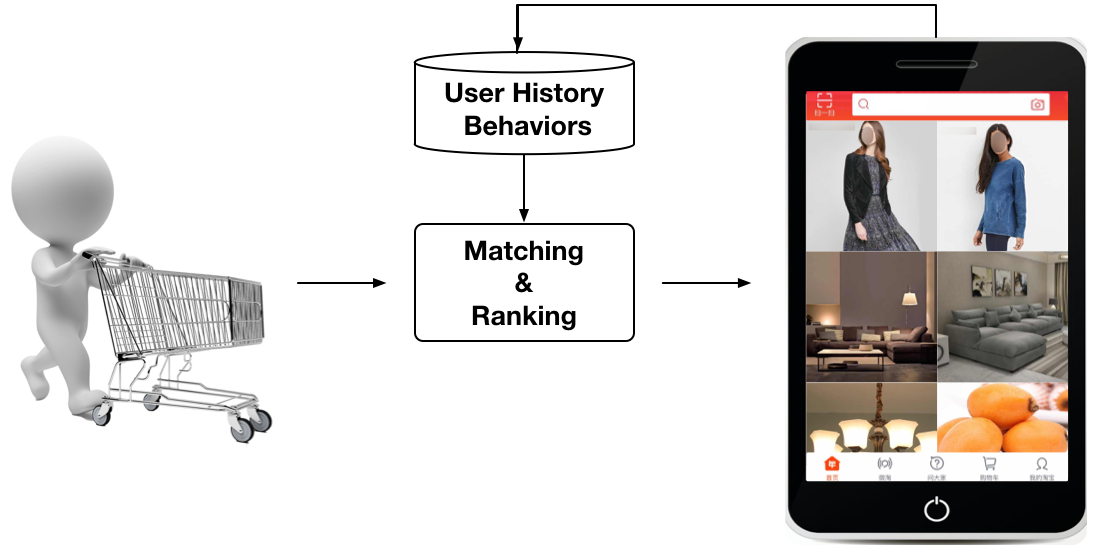
\includegraphics[height=2.5in, width=2.5in,keepaspectratio]{images/omni/sys4.png}
\caption{阿里巴巴展示广告系统运行流程示意图，其中用户行为数据发挥重要作用。}
\label{figure_display_ad_scenario}
\vspace{-0.4cm}
\end{figure}

 









%Our click model is designed for CTR prediction of display advertising. The observations of this application are Users' profile information, Ads' static attributes, and Users' behavior history. Different from the sponsored search, users come into display advertising system without clear target. Thus we wish to mining users' interest from the context information and estimate the CTR of each display accurately.
\section{深度兴趣网络}\label{sec:opa}

与赞助搜索不同，用户进入展示广告系统时并没有明确表达的意图。
构建 CTR 预测模型时，需要有效方法从丰富的历史行为中提取用户兴趣。
描述用户和广告的特征是广告系统 CTR 建模的基本元素。
合理使用这些特征并从中挖掘信息至关重要。

\subsection{特征表征}
工业 CTR 预测任务中的数据大多呈多组类别形式，例如 [weekday=Friday, gender=Female, \\ visited$\_$cate$\_$ids=$\{$Bag,Book$\}$, ad$\_$cate$\_$id=Book]，
通常会通过编码转换为高维稀疏二值特征 \cite{deep_crossing,widedeep,ftrl}。
在数学上，第 $i$ 个特征组的编码向量形式化为 $\textbf{t}_i \in R^{K_i}$。$K_i$ 表示特征组 $i$ 的维度，即特征组 $i$ 包含 $K_i$ 个唯一 id。
$\textbf{t}_i[j]$ 是 $\textbf{t}_i$ 的第 j 个元素，且 $\textbf{t}_i[j] \in \{0,1\}$。$\sum_{j=1}^{K_i} \textbf{t}_i[j]=k$。
当 $k=1$ 时，向量 $\textbf{t}_i$ 表示 one-hot 编码；当 $k>1$ 时，表示 multi-hot 编码。
随后，一个样本可以按组表示为 $\bs{x} = [\bs{t}_1^T, \bs{t}_2^T,...\bs{t}_M^T]^T$，其中 $M$ 为特征组数量，$\sum_{i=1}^{M}K_i = K$，$K$ 为整个特征空间的维度。
通过这种方式，上述包含四组特征的样本可表示为：
%\begin{equation}
\[
%  \underbrace{a + \overbrace{b+\cdots}^{{}=t}+z}_{\text{total}} ~~ a + {\overbrace{b+\cdots}^{126}+z
\underbrace{[0,0,0,0,1,0,0]}_{\text{weekday=Friday}} ~ \underbrace{[0,1]}_{\text{gender=Female}} ~ \underbrace{[0,..,1,...,1,...0]}_{\text{visited\_cate\_ids=\{Bag,Book\}}} 
~ \underbrace{[0,..,1,...,0]}_{\text{ad\_cate\_id=Book}}
\]
%\end{equation}

表 \ref{table_feature_set} 描述了我们系统中使用的完整特征集。
它由四类特征组成，其中用户行为特征通常是 multi-hot 编码向量，并包含丰富的用户兴趣信息。
需要注意的是，在我们的设置中没有组合特征。我们使用深度神经网络捕获特征之间的交互。

\begin{table}
\caption{阿里巴巴展示广告系统中使用的特征集统计。特征按组由稀疏二值向量组成。} % The dimensionality of fine-grained $goods\_ids$ feature scales up to $10^9$.}
\centering
\resizebox{0.47\textwidth}{!}{%
\label{table:fea-table}
\begin{tabular}{llccc}
\toprule
Category & Feature Group & Dimemsionality & Type & \#Nonzero Ids per Instance\\ \toprule
\multirow{3}{7em}{User Profile Features }
& gender & 2 &  one-hot & 1  \\ \cline{2-5}
& age\_level & $\sim 10$ &  one-hot & 1  \\ \cline{2-5}
& ... & ... & ... & ...  \\ \midrule

\multirow{4}{7em}{User Behavior Features}
& visited\_goods\_ids& $\sim 10^9$ &  multi-hot & $\sim 10^3$  \\ \cline{2-5}
& visited\_shop\_ids& $\sim 10^7$ &  multi-hot & $\sim 10^3$  \\ \cline{2-5}
& visited\_cate\_ids& $\sim 10^4$ &  multi-hot & $\sim 10^2$  \\\midrule

\multirow{4}{7em}{Ad Features }
& goods\_id & $\sim 10^7$ &  one-hot & 1  \\ \cline{2-5}
& shop\_id & $\sim 10^5$ &  one-hot & 1  \\ \cline{2-5}
& cate\_id & $\sim 10^4$ &  one-hot & 1   \\ \cline{2-5}
& ... & ... & ... & ...  \\ \midrule

\multirow{3}{7em}{Context Features }
& pid & $\sim 10$ &  one-hot & 1  \\ \cline{2-5}
& time & $\sim 10$ &  one-hot & 1  \\ \cline{2-5}
& ... & ... & ... & ...  \\ \bottomrule
\end{tabular}}
\label{table_feature_set}
\end{table}


\begin{figure*}[!t]
\centering
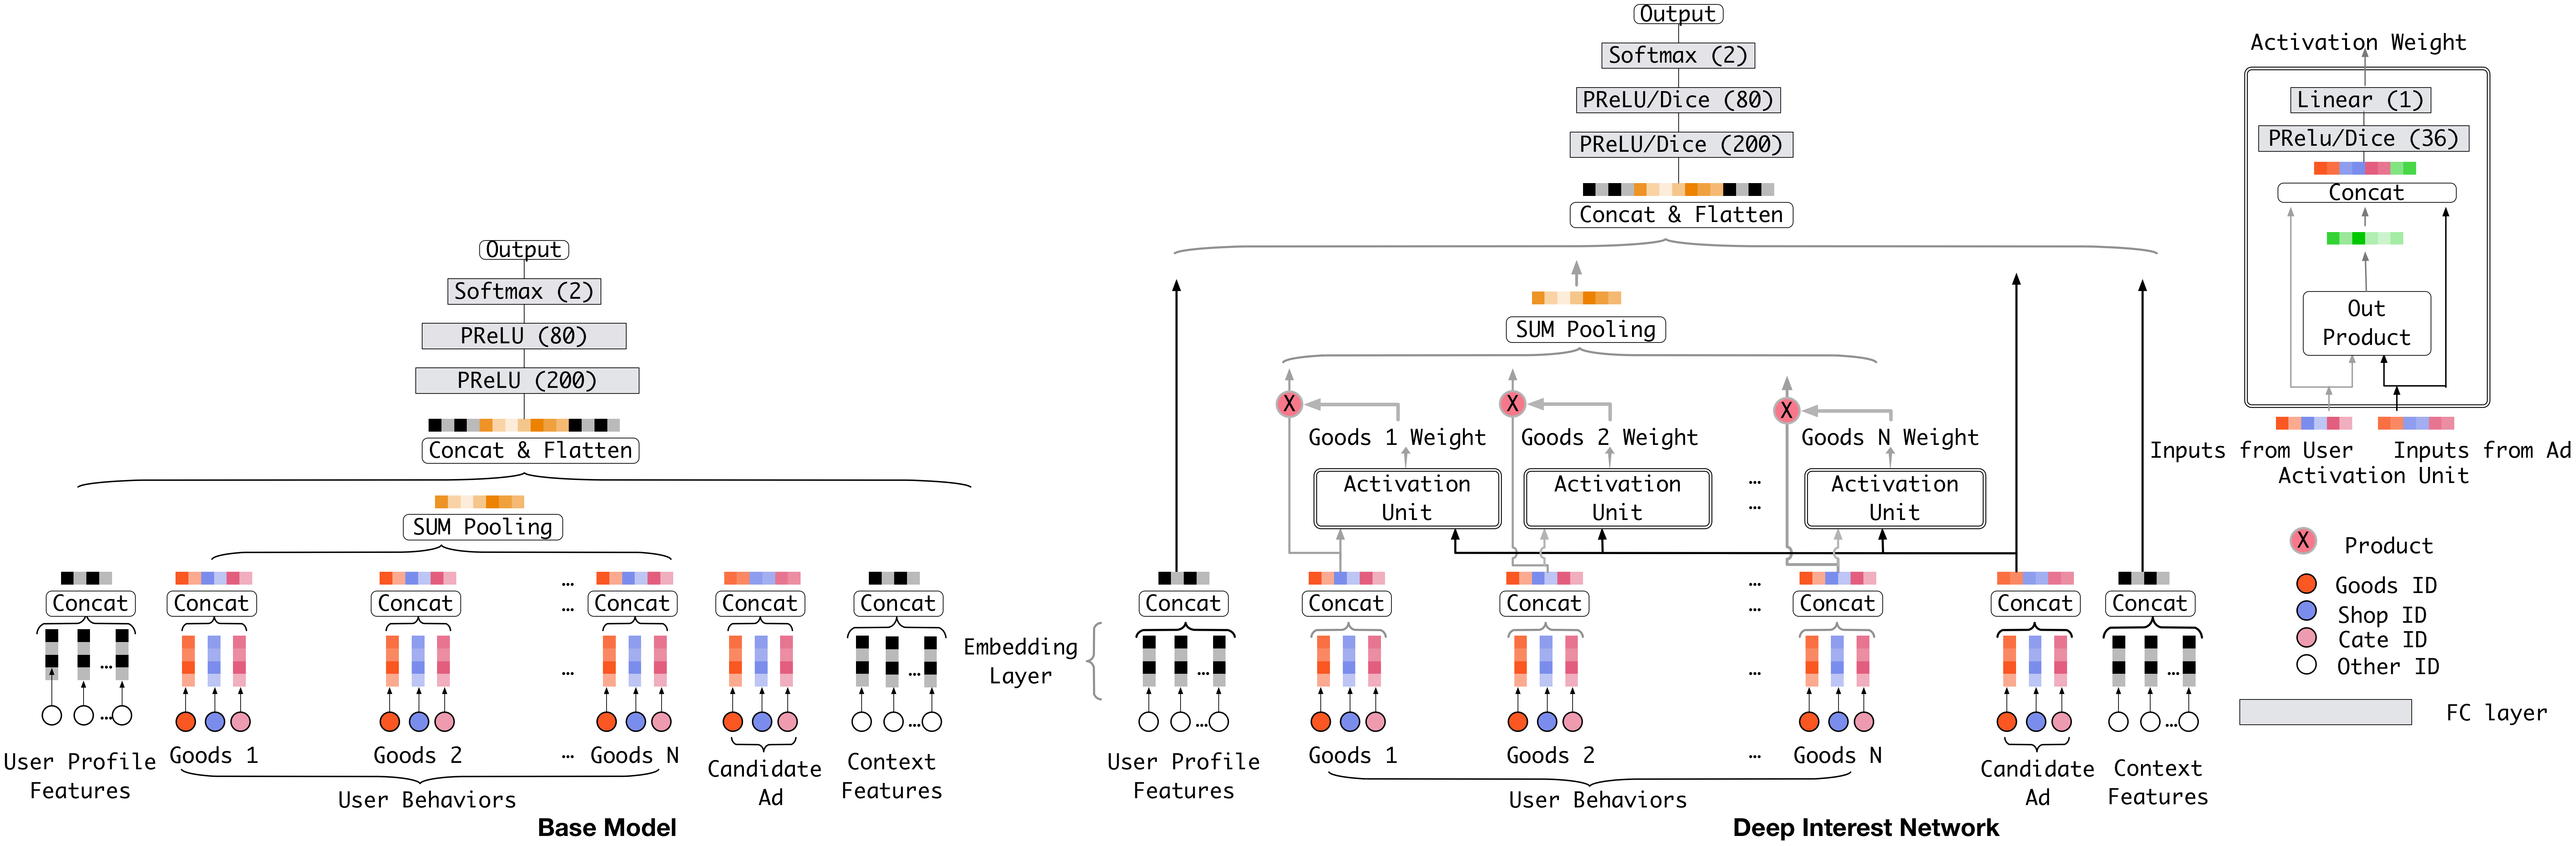
\includegraphics[height=7in, width=7in,keepaspectratio]{images/omni/DIN_new.png}
\caption{网络架构。左侧展示基础模型 (Embedding\&MLP) 的网络。属于同一商品的 cate\_id、shop\_id 和 goods\_id 的 embedding 被拼接起来，用于表示用户行为中的一个访问商品。右侧是我们提出的 DIN 模型。它引入局部激活单元，使用户兴趣表征能够针对不同候选广告自适应变化。}
\label{model_arch}
\end{figure*}


\subsection{基础模型 (Embedding\&MLP)}
\label{sec:basemodel}
%Following the popular model structure introduced in \cite{deep_crossing,widedeep,youtube:recommend}, we design our base model as shown in the left of Fig.\ref{model_arch}.
大多数流行模型结构 \cite{deep_crossing,widedeep,youtube:recommend} 共享相似的 Embedding\&MLP 范式，本文将其称为基础模型，如图 \ref{model_arch} 左侧所示。它由几个部分组成：
%It follows the embedding\&MLP architecture. %, with all the parameters trained in the end-to-end manner.
\paragraph{\textbf{Embedding 层}} 由于输入是高维二值向量，embedding 层用于将其转换为低维稠密表征。
%Let $\bs{t}_i\in \mathbb{R}^{K_i}$ represent the feature vector of i-th group in Table \ref{table_feature_set}. 
%Then one instance can be represent as $\bs{x} = [\bs{t}_1^T, \bs{t}_2^T,...\bs{t}_M^T]^T$ in a group-wise manner, where $M$ is number of feature groups, $\sum_{i=1}^{M}K_i = K$, $K$ is dimensionality of the entire feature space. 
对于 $\bs{t}_i$ 的第 $i$ 个特征组，令 $\mathrm{W}^i = [w_1^i,...,w_j^i, ..., w_{K_i}^i] \in\mathbb{R}^{D \times K_i}$ 表示第 $i$ 个 embedding 字典，其中 $w_j^i \in R^D$ 是维度为 $D$ 的 embedding 向量。
%Given instance of $\bs{x} = [\bs{t}_1^T, \bs{t}_2^T,...\bs{t}_M^T]^T$.
embedding 操作遵循查表机制，如图 \ref{model_arch} 所示。
\begin{itemize}
\item 如果 $\bs{t}_i$ 是 one-hot 向量，且第 j 个元素 $\bs{t}_i[j]=1$，则 $\bs{t}_i$ 的 embedding 表征是单个 embedding 向量 $\bs{e}_i = w_j^i$。
\item 如果 $\bs{t}_i$ 是 multi-hot 向量，且 $\bs{t}_i[j]=1 ~\text{for}~ j \in \{i_1, i_2, ..., i_k\} $，则 $\bs{t}_i$ 的 embedding 表征是一组 embedding 向量：$\{\bs{e}_{i_1}, \bs{e}_{i_2},...\bs{e}_{i_k}\} = \{w_{i_1}^i, w_{i_2}^i, ...w_{i_k}^i\}$。
\end{itemize}



\paragraph{\textbf{Pooling 层和 Concat 层}}
注意，不同用户拥有不同数量的行为。因此，multi-hot 行为特征向量 $\bs{t}_i$ 中非零值的数量会随样本变化，导致对应 embedding 向量列表的长度可变。
由于全连接网络只能处理定长输入，常见做法 \cite{widedeep,youtube:recommend} 是通过 pooling 层将 embedding 向量列表转换为定长向量：
\begin{equation}
\label{eq:pooling}
\bs{e}_i = \text{pooling}(\bs{e}_{i_1}, \bs{e}_{i_2},...\bs{e}_{i_k}).	
\end{equation}
最常用的两种 pooling 层是 sum pooling 和 average pooling，它们对 embedding 向量列表执行逐元素求和或求平均操作。

embedding 层和 pooling 层都按组操作，将原始稀疏特征映射为多个定长表征向量。
随后，将所有向量拼接起来，得到该样本的整体表征向量。

\paragraph{\textbf{MLP}} 给定拼接后的稠密表征向量，全连接层用于自动学习特征组合。
近期提出的方法 \cite{widedeep,DeepFM,PNN} 关注 MLP 结构设计，以更好地提取信息。\par
\paragraph{\textbf{损失}}基础模型使用的目标函数是负对数似然函数，定义如下：
\begin{equation}
    L= - \frac{1}{N} \sum_{(\bs{x},y)\in\mathcal{S}} (y\log p(\bs{x}) + (1-y)\log(1-p(\bs{x}))),
\end{equation}
其中 $\mathcal{S}$ 是大小为 $N$ 的训练集，$\bs{x}$ 是网络输入，$y\in \{0,1\}$ 是标签，$p(\bs{x})$ 是网络经过 softmax 层后的输出，表示样本 $\bs{x}$ 被点击的预测概率。


\subsection{深度兴趣网络结构}

在表 \ref{table_feature_set} 的所有特征中，用户行为特征至关重要，并在电商应用场景中的用户兴趣建模中发挥关键作用。

基础模型通过对用户行为特征组中的所有 embedding 向量进行 pooling，获得用户兴趣的定长表征向量，如式 (\ref{eq:pooling}) 所示。对于给定用户，无论候选广告是什么，该表征向量都保持不变。
通过这种方式，维度有限的用户表征向量会成为表达用户多样化兴趣的瓶颈。
为了使其具备足够能力，一个简单方法是扩展 embedding 向量的维度，但这会显著增加学习参数规模。
在训练数据有限时，这会导致过拟合，并增加计算和存储负担，而工业级在线系统可能无法承受这些开销。

%As discussed above, when visiting e-commerce sites, users are often interested in many kinds of goods. 
%In other words, user interests are diverse.  
%However, it is known that users are often with diverse interests when visiting e-commerce sites. 
%Base model obtains the user interest vector by average pooling over the embedding of all behaviors. Thus base model obtains a same interest vector of users given different candidate ads for one user.
% In the base model, sums the embedding of all user behavior ids to obtain the user interest vector. The model obtains the same user % interest vector when predicts different candidate ad for one user.
%In order to embed diverse user interests in this vector, one easy method is expanding the dimension to make it capable enough to contain information of different interests. 
%Unfortunately, high dimension of embedding vectors will increase the size of learning parameters heavily.
%It will lead to overfitting under limited training data and add the burden of computation and storage, which may not be tolerated for an industrial online system.

是否存在一种优雅方式，能够在有限维度下用一个向量表示用户的多样化兴趣？
用户兴趣的局部激活特征启发我们设计了一种名为深度兴趣网络 (DIN) 的新模型。
设想第 \ref{sec:bg} 节中提到的年轻母亲访问电商网站时，看到展示的新手提包很可爱并点击了它。
我们分析这一点击行为的驱动力。
所展示的广告通过软搜索她的历史行为，并发现她近期浏览过相似的托特包和皮质手提包商品，从而命中了这位年轻母亲的相关兴趣。
换言之，与展示广告相关的行为对点击动作有很大贡献。
DIN 通过关注相对于给定广告的局部激活兴趣表征来模拟这一过程。
DIN 不使用同一个向量表达用户的全部多样化兴趣，而是考虑历史行为相对于候选广告的相关性，自适应计算用户兴趣表征向量。
该表征向量会随广告不同而变化。

图 \ref{model_arch} 右侧展示了 DIN 的架构。
与基础模型相比，DIN 引入了新设计的局部激活单元，并保持其他结构不变。具体而言，激活单元应用于用户行为特征，在给定候选广告 $A$ 时执行加权求和池化，以自适应计算用户表征 $\bs{v}_U$，如式 (\ref{eq:attention}) 所示。


%By simulating this process, we   
%Instead of focusing on a global representation vector, we actually only need to pay attention to the representation of locally related interests given a candidate ad.  
%In this way, representation vector of user interest is calculated adaptively given $\prec$user, ad$\succ$ pair. 
%That is, it varies over different candidate ads.  
%Then user vector only needs to represent related interest when faced different candidate ad, which is within the ability of a vector with appropriate dimension. \par
%For different candidate ads, we want our model to find related part of interests automatically. \par
%This candidate specific interest vector can be realized by attention mechanism\cite{bengio:attention}, which derive from neural machine translation.
%Under this consideration, we design a novel model named deep interest network(DIN), to better capture the characteristic of user behavior data and help improving the expressive ability of model under limited embedding dimension. 
%It is illustrated in the right of Fig.\ref{model_arch}.
%Compared with base model, DIN introduces a new designed activation unit and maintains the other net structures the same.  

%Specifically, activation unit is applied on the user behavior feature groups, which performs as a weighted average pooling to adaptively calculate user representation $\bs{v}_U$ given a candidate ad $A$, as shown in Eq.(\ref{eq:attention})
{
%\setlength\abovedisplayskip{1pt}
%\setlength\belowdisplayskip{1pt}
\begin{small}
\begin{equation}
\begin{split}
\label{eq:attention}
\bs{v}_U(A) = f(\bs{v}_A,\bs{e}_1,\bs{e}_2,..,\bs{e}_H) & = \sum_{j=1}^H a(\bs{e}_j,\bs{v}_A) \bs{e}_j = \sum_{j=1}^H \bs{w}_j \bs{e}_j,
\end{split}
\end{equation}
\end{small}
}
其中 $\{\bs{e}_1, \bs{e}_2, ..., \bs{e}_H\}$ 是用户 $U$ 的行为 embedding 向量列表，长度为 $H$，$\bs{v}_A$ 是广告 $A$ 的 embedding 向量。通过这种方式，$\bs{v}_U(A)$ 会随广告不同而变化。$a(\cdot)$ 是一个前馈网络，其输出作为激活权重，如图 \ref{model_arch} 所示。除两个输入 embedding 向量外，$a(\cdot)$ 还加入它们的外积并输入后续网络，这是一种有助于相关性建模的显式知识。

式 (\ref{eq:attention}) 中的局部激活单元与 NMT 任务中发展的注意力方法 \cite{bengio:attention} 具有相似思想。
然而，与传统注意力方法不同，式 (\ref{eq:attention}) 放宽了 $\sum_i w_i = 1$ 约束，目的是保留用户兴趣强度。
也就是说，我们舍弃了对 $a(\cdot)$ 输出进行 softmax 归一化。
相反，$\sum_i w_i$ 的值在一定程度上被视为激活用户兴趣强度的近似。
例如，如果某个用户的历史行为中 90\% 是服装，10\% 是电子产品。
给定 T 恤和手机两个候选广告，T 恤会激活大多数属于服装的历史行为，并可能比手机得到更大的 $\bs{v}_U$ 值，即更高的兴趣强度。
传统注意力方法通过归一化 $a(\cdot)$ 的输出，会丢失 $\bs{v}_U$ 数值尺度上的分辨率。
%Taking the original output of $a(\cdot)$  as activation score can be a simple way to maintain the intensity of interest, which helps making use of user historical behavior data more sufficiently.


%Assume user U is interested in clothes and electronics, with the intensity to be 90\% and 10\% relatively. 
%This causes the historical behaviors of clothes occur more \textbf{frequently} than electronics for $U$.     
%Assume two candidate ads T-shirt and iphone are selected as candidates for $U$.
%Value of representation vector $\bs{v}_U$ given T-shirt will be larger than given iphone.
%Indeed, taking the original output of $a(\cdot)$  as activation weight can be a simple way to maintain the intensity of interest, which helps us making use of user historical behavior more sufficiently.

我们尝试过用 LSTM 以序列方式建模用户历史行为数据。
但它没有带来提升。
%But it makes little difference. 
不同于 NLP 任务中受语法约束的文本，用户历史行为序列可能包含多个并发兴趣。
这些兴趣之间的快速跳转和突然终止会使用户行为序列数据显得有噪声。
一个可能方向是设计特殊结构，以序列方式建模这类数据。
我们将其留作未来研究。


%Meanwhile, user behavior is not only affected by his diverse interests but also depends on the results our system display. 
%In our attempt, directly modeling user behavior sequence with RNNs shows little improvement.  
%This makes it difficult for directly deploying the RNNs to model user behavior sequence in e-commerce scenario.

%It's notable that the value of $\bs{v}_U$ given candidate ad that relates to \textbf{frequent} historical behavior is larger than others. 
%For example, if one user's historical behavior contains 80\% clothes and 20\% electronics. For candidate ads: T-shirt and phone, more historical behaviors get high attention score for T-shirt, which leads to the value of vector $\bs{v}_U$ computed for the user is larger for T-shirt than for phone. It means the value of vector can reflect the user's interest intensity. But traditional attention methods that use normalization with softmax on the output of $a$ to scale the value of $\bs{v}_U$ into the same range is not suitable in our scenario, which may lose the information of interest intensity. Instead, the original output of $a$ can maintain the intensity of interest, which helps us making use of user historical behavior more sufficiently.

%It seems to be natural to use RNNs for modeling user interest by taking the sequence of user behaviors as inputs. 
%However, we implement it and find no difference. 
%A possible explanation is that different from text that is under the constraint of grammar, the sequence of user historical behaviors contains concurrent multiple varying interests and may rapidly jump over these interests, which make the sequence data to be disordered and noisy. 
%We leave this for future research. 
%Meanwhile, user's behavior is not only affected by his diverse interests but also another factors such as the results our system display. Thus the information about sequence in e-commerce scenario is much weaker than that in text.
 

%The use of attention makes users' diverse interest be captured. Further, these diversity interest can be local activated when predict one specific candidate ad.
%In all, DIN designs the activation unit to follow local activation structure and weighted sum pooling to follow diversity structure.
%To the best of our knowledge, DIN is the first model which follows both of the two structures of user behavior data in CTR prediction tasks at the same time.
%\subsection{Mini-batch Aware Regularization Technique}

\section{训练技术}
在阿里巴巴广告系统中，商品和用户数量规模达到数亿。
%There are billion kinds of goods in Alibaba, and our advertising system needs to serve more than hundred million users one day.
实际中，使用大规模稀疏输入特征训练工业级深度网络具有很大挑战。
本节介绍两项在实践中被证明有帮助的重要技术。

\subsection{Mini-batch Aware 正则化}

%In order to capture more specific interests of users, we typically introduce billions of fine-grained ids to describe the users' behaviors. These sparse and high dimensional features may lead to severe overfitting problem.
%{\EDIT why these feature would cause overfitting?(1 more parameter ; 2 less times)}
%to capture user interest detailly. \par
%Not surprisingly, overfitting problem is encountered while training our model with large scale parameters and sparse inputs.
%In experiment, with addition of fine-grained user visited $good\_ids$ feature, model performance falls rapidly after the first epoch.\par
%It is known that internet-scale user behavior data follows the long-tail law, that is, lots of feature ids occur a few times in the training samples, while little of them occur many times.
%This inevitably introduces noise into the training process and intensifies overfitting.
%An easy way to reduce overfitting is to filter out those low-frequency feature ids, which can be viewed as manual regularization.
%However, such frequency based filter is quite rough in terms of information loss and threshold setting.
%Many methods have been proposed to reduce overfitting, such as $\ell_2$ and $\ell_1$ regularization \cite{lasso}, and Dropout \cite{dropout}. 
%However, merely of them are suitable for training network with sparse inputs and billions of parameters.

%Practically overfitting problem is encountered while training industrial networks with large scale sparse input features.
过拟合是训练工业级网络的关键挑战。
例如，加入细粒度特征后，如维度为 6 亿的 $\textsl{goods\_ids}$ 特征，包括表 \ref{table_feature_set} 中描述的用户 $visited\_goods\_ids$ 和广告 $goods\_id$，如果训练时不使用正则化，模型性能会在第一个 epoch 后迅速下降，如后文第 \ref{sec:reg} 节图 \ref{fig:adaptive_reg} 中的深绿色曲线所示。
对于稀疏输入且包含数亿参数的网络，直接使用传统正则化方法并不现实，例如 $\ell_2$ 和 $\ell_1$ 正则化。
以 $\ell_2$ 正则化为例。
在没有正则化的基于 SGD 的优化方法中，每个 mini-batch 只需要更新出现的非零稀疏特征参数。
然而，加入 $\ell_2$ 正则化后，每个 mini-batch 都需要在全部参数上计算 L2-norm，这会产生极重的计算开销，当参数规模达到数亿时不可接受。
%Original $\ell_2$ regularization needs to calculated L2-norm over the whole parameters on each mini-batch, which leads to extremely heavy computations and is unacceptable in our situation. 

\begin{figure}[!ht]
%\setlength{\belowcaptionskip}{-0.5cm}
\centering
%\includegraphics[height=4.5in, width=5in,keepaspectratio]{images/omni/system}
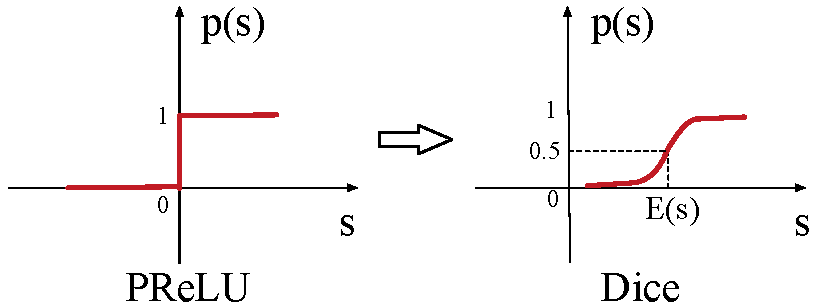
\includegraphics[height=1.8in, width=2.2in,keepaspectratio]{images/omni/dice_activation}
\caption{PReLU 和 Dice 的控制函数。}
\label{figure_dice}
\vspace{-0.4cm}
\end{figure} 


本文提出了一种高效的 mini-batch aware 正则化器，它只对每个 mini-batch 中出现的稀疏特征参数计算 L2-norm，从而使计算可行。
事实上，CTR 网络的大部分参数来自 embedding 字典，也正是它带来了沉重计算的困难。
令 $\bs{\mathrm{W}}\in\mathbb{R}^{D\times K}$ 表示整个 embedding 字典的参数，其中 $D$ 是 embedding 向量维度，$K$ 是特征空间维度。
在样本上展开 $\bs{\mathrm{W}}$ 的 $\ell_2$ 正则化：
%\begin{equation}
%\label{eq:batch}
%\sum_{i=1}^{n_{dj}} \frac{I_{id}}{n_{dj}}w_d^2
%\end{equation}
\begin{footnotesize}
\begin{equation}
\begin{split}
\label{eq:batch}
L_2(\bs{\mathrm{W}}) &= \|\bs{\mathrm{W}}\|_2^2 = \sum_{j=1}^{K}\|\bs{w}_j\|_2^2 = \sum_{(\bs{x},y)\in\mathcal{S}}\sum_{j=1}^{K} \frac{I(\bs{x}_j\neq0)}{n_{j}}\|\bs{w}_j\|_2^2,
\end{split}
\end{equation}
\end{footnotesize}
其中 $\bs{w}_j\in\mathbb{R}^{D}$ 是第 $j$ 个 embedding 向量，
%which corresponding to the number of feature IDs in our applications.
$I(\bs{x}_j\neq0)$ 表示样本 $\bs{x}$ 是否具有特征 id $j$，$n_j$ 表示特征 id $j$ 在所有样本中的出现次数。%Here we use $I(\cdot)$ as the indicator function.
%When applying the gradient descent optimization on mini-batches, the regularization is transformed into
式 (\ref{eq:batch}) 可以按 mini-batch aware 方式转换为式 (\ref{eq:minibatch})：
\begin{small}
\begin{equation}
\label{eq:minibatch}
L_2(\bs{\mathrm{W}}) = \sum_{j=1}^{K}\sum_{m=1}^{B}\sum_{(\bs{x},y)\in\mathcal{B}_m}\frac{I(\bs{x}_j\neq 0)}{n_{j}}\|\bs{w}_j\|_2^2,
\end{equation}
\end{small}
其中 $B$ 表示 mini-batch 的数量，$\mathcal{B}_m$ 表示第 $m$ 个 mini-batch。
%To simplify the computation, 
令 $\alpha_{mj} = \max_{(\bs{x},y)\in\mathcal{B}_m} I(\bs{x}_j\neq0)$
%{\small
%\begin{equation}
%\alpha_{mj} = \max_{(\bs{x},y)\in\mathcal{B}_m} I(\bs{x}_j\neq0),
%\end{equation}}
表示 mini-batch $\mathcal{B}_m$ 中是否至少有一个样本包含特征 id $j$。
则式 (\ref{eq:minibatch}) 可以近似为：
\begin{small}
\begin{equation}
\label{eq:approx}
L_2(\bs{\mathrm{W}})\approx\sum_{j=1}^{K} \sum_{m=1}^{B}  \frac{\alpha_{mj}}{n_j}\|\bs{w}_j\|_2^2.
\end{equation}
\end{small}
通过这种方式，我们推导出了 $\ell_2$ 正则化的近似 mini-batch aware 版本。
对于第 $m$ 个 mini-batch，关于特征 $j$ 的 embedding 权重的梯度为：
%\begin{equation}	
%\scalebox{0.9}{
%\parbox{0.37\textwidth}{
%\begin{eqnarray}
%\begin{split}
%\bs{w}_j \leftarrow \bs{w}_j- \eta
%    \left[
%       \frac{1}{|\mathcal{B}_m|} \sum_{(\bs{x},y) \in \mathcal{B}_m} { \frac{\partial L(p(\bs{x}), y)}{\partial \bs{w}_j}
%       +\lambda \frac{\alpha_{mj}}{n_j}\bs{w}_j}
%    \right].
%\end{split}
%\end{eqnarray}
%}
%}
%\end{equation}
\begin{small}
\begin{equation}
\bs{w}_j \leftarrow \bs{w}_j- \eta
    \left[
       \frac{1}{|\mathcal{B}_m|} \sum_{(\bs{x},y) \in \mathcal{B}_m} { \frac{\partial L(p(\bs{x}), y)}{\partial \bs{w}_j}
       +\lambda \frac{\alpha_{mj}}{n_j}\bs{w}_j}
    \right],
\end{equation}
\end{small}
其中只有出现在第 $m$ 个 mini-batch 中的特征参数参与正则化计算。

%Different from the regularization in~\cite{difacto}, our approach imposes more penalty on long-tail features(which is hard to learn) of lower frequency than frequent $goods\_id$(which may reflect user interests confidently). 
%Experiments show that our approach outperforms other regularization methods, like dropout.




% let $w_j$ denotes the parameter in embedding layer,
%In common, the gradient of loss  $L(x; W)$ combined with $L_2(W)$ to the embedding layer's parameter $W_{jk}$(the embedding matrix for the kth id of feature $X_j$)is
%\begin{equation}
%\label{ada-reg}
%W_{jk} \leftarrow W_{jk} - \eta
%    \left[
%       \frac{1}{b} \sum_{(x_i,y_i) \in B} { \frac{\partial L(f(x_i), y_i)}{\partial W_{jk}} +\lambda W_{jk}}
%    \right]
%\end{equation}
%Where $B$ stands for mini-batch samples with size of $b$.  $\lambda$ is regularization parameter.

%Many methods have been proposed to reduce overfitting, such as $L_2$ and $L_1$ regularization \cite{lasso}, and Dropout \cite{dropout}.
%However, with sparse and high dimensional data,  CTR prediction task faces greater challenge.
%It is known that internet-scale user behavior data follows the long-tail law, that is, lots of feature ids occur a few times in the training samples, while little of them occur many times.
%This inevitably introduces noise into the training process and intensifies overfitting.
%
%%According to our experience,
%An easy way to reduce overfitting is to filter out those low-frequency feature ids, which can be viewed as manual regularization.
%However, such frequency based filter is quite rough in terms of information loss and threshold setting.
%Here we introduce an adaptive regularization method, in which we impose different regularization intensity on feature ids according to their occurrence frequency.
%On realizing this method, we apply frequency related L2-norm regularization to good ids that actually occur in current mini-batch.
%The last term brings to some problem, on the one hand, it has effect on $W_{jk}$ even if $x_{ij}$ is 0. On the one hand, it improves the consumption of computation; On the other hand, it will lead error director for the update of $w_{e_j}$.\par
%
%In order to avoid extra updating, we try to introduce one control unit to the update when one batch using one specific id.
%Denote that,
%\begin{equation}
%I_i = \left\{ \begin{array}{ll}
%1, & \exists  (x_j,y_j) \in B, s.t. \left[ x_j \right]_i \neq 0\\
%0, & \textrm{other wises}
%\end{array} \right.
%\end{equation}
%
%\begin{equation}
%\label{ada-reg}
%W_{jk} \leftarrow W_{jk} - \eta
%    \left[
%       \frac{1}{b} \sum_{(x_i,y_i) \in B} { \frac{\partial L(f(x_i), y_i)}{\partial W_{jk}} +\lambda W_{jk}I_i}
%    \right]
%\end{equation}
% While there is another problem, the update times for different frequent feature is different, which means the regularization on low frequent feature is weak, which violates the goal.\par
% Aiming to solve this problem, we design an adaptive regularization method, which applies different regularization intensity on feature ids according to their occurrence frequency.
%Let's analyze the gradient updating from the aspect of instance.
%Aiming to solving this problems, we design an adaptive regularization method, which imposes different regularization intensity on feature ids according to their occurrence frequency.\par
%Denote that,
%\begin{equation}
%I_i = \left\{ \begin{array}{ll}
%1, & \exists  (x_j,y_j) \in B, s.t. \left[ x_j \right]_i \neq 0\\
%0, & \textrm{other wises}
%\end{array} \right.
%\end{equation}

%\begin{equation}
%\label{ada-reg}
%W_{jk} \leftarrow W_{jk} - \eta
%    \left[
%       \frac{1}{b} \sum_{(x_i,y_i) \in B} { \frac{\partial L(f(x_i), y_i)}{\partial W_{jk}} +\lambda \frac{1}{n_i}W_{jk}I_i}
%    \right]
%\end{equation}
%where $n_i$ is frequency of feature $i$.\par


%The idea behind Eq.(\ref{ada-reg}) is to penalize low-frequency features and relax high-frequency features to control the gradient update variance.
%When b is set to 1, the update is equivalent to dividing regularization term of full batch update onto each sample. When mini batch size is large than 1, we still use $\lambda \frac{1}{n_i}$ as regular coefficient to avoid counting good id's frequency in current mini batch.

%% PLAN A
%A similar practice of adaptive regularization can be found in \cite{difacto} which sets regular coefficient to be proportional to feature frequency where they
%, as shown below:
%\begin{equation}
%\label{limu}
%w_i \leftarrow w_i - \eta
%    \left[
%       \frac{1}{b} \sum_{(x_j,y_j) \in B} { \frac{\partial L(f(x_j), y_j)}{\partial w_i} +\lambda n_iw_iI_i}
%    \right]
%\end{equation}
%However, in our dataset, training with regularization of Eq.(\ref{limu}) shows no obvious alleviation of overfitting. On the contrary, it slows down the convergence of training process. Eq.(\ref{limu}) applies greater penalty on high-frequency good ids than long-tail goods, while the former contributes more on both the metric and online income in our special e-commerce system. Besides, we also evaluate dropout technique and find slight improvement on overfitting.
%However, when we train DNN model on our display advertisement data using the above equation, we could not observe the alleviation of overfitting. On the contrary, it slows down the convergence of training process, because of greater penalty on high-frequency good ids. We have also tested the case in which all good ids share the same regular coefficient, in other words, regular coefficient has no relationship with item frequency. In that case, overfitting still exists and the speed of convergence also slows down.
%\end{comment}


\subsection{数据自适应激活函数}
%{\EDIT
%In order to make DIN to be more suitable for industrial-scale net sparse input, besides the design of net structure and choice of input, we propose a new activation function to accelerate the convergence.

%Industrial-scale dimensionality of sparse features and data size give challenges to the convergence for training deep networks. 
%To fit the data better, we propose a data adaptive activation function to help convergence.



PReLU \cite{ms:prelu} 是一种常用激活函数：
\begin{small}
\begin{equation}
f(s) = \begin{cases}
       s & \text{ if } s > 0  \\
       \alpha s & \text{ if } s \leq 0.
       \end{cases}
     = ~ p(s) \cdot s + (1-p(s))\cdot \alpha s,   
\end{equation}
\end{small}
其中 $s$ 是激活函数 $f(\cdot)$ 输入的一维，$p(s) = I(s>0)$ 是指示函数，用于控制 $f(s)$ 在 $f(s)=s$ 和 $f(s)=\alpha s$ 两个通道之间切换。第二个通道中的 $\alpha$ 是学习参数。
这里我们将 $p(s)$ 称为控制函数。图 \ref{figure_dice} 左侧绘制了 PReLU 的控制函数。
PReLU 采用值为 $0$ 的硬整流点，当各层输入服从不同分布时，这可能并不合适。
考虑到这一点，我们设计了一种新的数据自适应激活函数，命名为 \textsl{\textbf{Dice}}：
\begin{equation}
f(s) = p(s) \cdot s + (1-p(s))\cdot \alpha s, \ \ p(s) = \frac{1}{ 1 + e^{- \frac{s - E[s]}{\sqrt{Var[s] + \epsilon}}}}
\end{equation}
其控制函数绘制在图 \ref{figure_dice} 右侧。
在训练阶段，$E[s]$ 和 $Var[s]$ 是每个 mini-batch 中输入的均值和方差。
在测试阶段，$E[s]$ 和 $Var[s]$ 由数据上的移动平均 $E[s]$ 和 $Var[s]$ 计算得到。
$\epsilon$ 是一个很小的常数，在我们的实践中设为 $10^{-8}$。

Dice 可以看作 PReLU 的一种推广。
Dice 的核心思想是根据输入数据分布自适应调整整流点，其值设为输入均值。
此外，Dice 以平滑方式控制两个通道之间的切换。
当 $E(s)=0$ 且 $Var[s]=0$ 时，Dice 退化为 PReLU。



%The key idea of Dice is to adaptively adjust the rectifier point according to data, which is different from PReLU.
%Instead of using a hard rectifier based on whether y is larger than 0,
%Dice adjusts the rectifier point by portion of $p$ which contains information of the mean and variance of inputs.
%It can be viewed as a soft rectifier with two channel: $\alpha y$ and $y$. $p$ is a adaptive weight. 

%PReLU plays the role as the Leaky ReLU to avoid zero gradients \cite{Mass:Lrelu} while the $a_i$ is small.
%Previous research has shown that PReLU can improve accuracy while with a little extra risk of overfitting.
%However, in our application with large scale sparse inputs, training such industrial-scale network  still faces a lot of  challenges.
%All variants of ReLU choose $0$ as the rectifier point. 
%However a hard rectifier point may be not suitable as the distribution of each layers's input is different.
%To further improve the convergency and performance of our model, 
%Hence, we design a novel data adaptive activation function, which we name Dice:
%\begin{align}
%f(\bs{y}_{k}) & = \bs{a}_{(k)}(1 - \bs{p}_{k})\bs{y}_{k} + \bs{p}_{k}\bs{y}_{k} \\
%\bs{p}_{k} & = \frac{1}{ 1 + e^{- \frac{\bs{y}_{k} - E[\bs{y}_{k}]}{\sqrt{Var[\bs{y}_{k}] + \epsilon}}}}
%\end{align}
%\begin{small}
%{\small
%\begin{equation}
%f(y) = \alpha(1 - p)y + py, \ \ p = \frac{1}{ 1 + e^{- \frac{y - E[y]}{\sqrt{Var[y] + \epsilon}}}}.
%\end{equation}In the training phrase, $E[y]$ and $Var[y]$ is the mean and variance of input of the nonlinear activation $f$ in one mini batch, with $\epsilon=10^{-8}$. In the testing phrase, $E[y]$ and $Var[y]$ is computed by moving averages $E[y]$ and $Var[y]$ in training processing. 
%In testing phrase, we adopt the momentum method to estimate the running ${E[y]}^{'}$ and ${Var[y]}^{'}$:
%
%\begin{align}
%{E[y]_{t+1}}^{'} & = (1-\alpha){E[y]_{t}}^{'} + \alpha {E[y]}_{t+1}\\
%{Var[y]_{t+1}}^{'} & = (1-\alpha){Var[y]_{t}}^{'} + \alpha {Var[y]}_{t+1}
%\end{align}
%$t$ is the mini batch step of the training process, and $\alpha$ is a super parameter like 0.99. In the test step we used the running ${E[y_{i}]}^{'}$ and ${Var[y_{i}]}^{'}$.

%In testing phrase, the weighted average of last two batch's mean and variance in training are used  mean and variance:
%\begin{align}
%{E[y]_{t}}^{'} & = (1-\alpha){E[y]_{t-1}}^{'} + \alpha {E[y]}_{t}\\
%{Var[y]_{t}}^{'} & = (1-\alpha){Var[y]_{t-1}}^{'} + \alpha {Var[y]}_{t}
%\end{align}

%The key idea of Dice is to adaptively adjust the rectifier point according to data, which is different from PReLU.
%Instead of using a hard rectifier based on whether y is larger than 0,
%Dice adjusts the rectifier point by portion of $p$ which contains information of the mean and variance of inputs.
%It can be viewed as a soft rectifier with two channel: $\alpha y$ and $y$. $p$ is a adaptive weight. 
%Experiments show Dice provides an obviously improvement on convergency.



%\subsection{Deep Interest Network}
%\label{din}

\section{实验} \label{exp}
%In this section, We first compare DIN with other methods including Wide\&Deep\cite{widedeep}, PNN\cite{PNN}, deepFM\cite{DeepFM} and Logistic Regression on two public dataset. DINs need to be evaluated on dataset with user behaviors, but not all dataset about CTR prediction contains user behaviors. Two public datasets with user behaviors: Amazon Dataset\footnote{http://jmcauley.ucsd.edu/data/amazon/} and MovieLens\footnote{https://grouplens.org/datasets/movielens/20m/} are used in this paper. Then our proposed methods are evaluated on Alibaba product data. We evaluate the effectiveness of the proposed structure of Deep Interest Network, activation function: Dice as well as the Mini-batch Aware Regularization Technique.

%In this section, we conduct empirical study on the performance of proposed DIN model and training techniques.
本节详细介绍实验，包括数据集、评价指标、实验设置、模型比较以及相应分析。
在两个包含用户行为的公开数据集以及从阿里巴巴展示广告系统采集的数据集上的实验表明，所提方法有效，并且在 CTR 预测任务上优于 SOTA 方法。
公开数据集和实验代码均已开放\textsuperscript{\ref{code}}。%\footnote{Experiment codes on two public datasets are available at GitHub: https://github.com/zhougr1993/DeepInterestNetwork}.

\subsection{数据集与实验设置}
\textbf{Amazon Dataset\footnote{http://jmcauley.ucsd.edu/data/amazon/}.}
Amazon Dataset 包含来自 Amazon 的商品评论和元数据，被用作基准数据集\cite{Amazon:AUC,AmazonData,ICCV_Amazon}。我们在名为 Electronics 的子集上进行实验，该子集包含 192,403 个用户、63,001 个商品、801 个类别和 1,689,188 个样本。该数据集中的用户行为较为丰富，每个用户和商品都有超过 5 条评论。特征包括 goods\_id、cate\_id、用户评论过的 goods\_id\_list 和 cate\_id\_list。设某个用户的全部行为为 ($b_1, b_2, \ldots, b_k, \ldots, b_n$)，任务是利用前 k 个评论过的商品预测第 (k+1) 个评论商品。
    对每个用户，使用 $k = 1, 2, \ldots, n - 2$ 生成训练数据集。在测试集中，我们给定前 $n-1$ 个评论商品来预测最后一个。
    对所有模型，我们使用带指数衰减的 SGD 作为优化器，其中学习率从 1 开始，衰减率设为 0.1。%We also tried Adam\cite{Adam}, which provides faster convergency but brings worse results than SGD for all deep models.
    mini-batch 大小设为 $32$。

    
\textbf{MovieLens Dataset\footnote{https://grouplens.org/datasets/movielens/20m/}.} MovieLens 数据\cite{MovieLens} 包含 138,493 个用户、27,278 部电影、21 个类别和 20,000,263 个样本。为了使其适用于 CTR 预测任务，我们将其转换为二分类数据。原始用户电影评分是 0 到 5 之间的连续值。我们将评分为 4 和 5 的样本标记为正样本，其余标记为负样本。我们根据 userID 将数据划分为训练数据集和测试数据集。在全部 138,493 个用户中，随机选择 100,000 个进入训练集，约 14,470,000 个样本，其余 38,493 个进入测试集，约 5,530,000 个样本。任务是基于历史行为预测用户是否会给定某部电影超过 3 分，即正标签。特征包括 movie\_id、movie\_cate\_id 以及用户评分过的 movie\_id\_list、movie\_cate\_id\_list。我们使用与 Amazon Dataset 相同的优化器、学习率和 mini-batch 大小。

\textbf{Alibaba Dataset.} 我们从阿里巴巴在线展示广告系统采集流量日志，其中两周的样本用于训练，随后一天的样本用于测试。训练集和测试集大小分别约为 20 亿和 1.4 亿。对于所有深度模型，全部 16 组特征的 embedding 向量维度均为 12。%So the input dimension of first layer in MLP is 192.
MLP 层设置为 $192 \times 200 \times 80 \times 2$。由于数据规模巨大，我们将 mini-batch 大小设为 5000，并使用 Adam\cite{Adam} 作为优化器。我们采用指数衰减，其中学习率从 0.001 开始，衰减率设为 0.9。

上述所有数据集的统计信息如表 \ref{table:Statistics} 所示。
Alibaba Dataset 的规模远大于 Amazon 和 MovieLens，因此带来了更多挑战。

    
\begin{table}[!t]
%\setlength{\belowcaptionskip}{-1cm}
\caption{本文使用的数据集统计。}
\small
\centering
\begin{threeparttable}
\begin{tabular}{lcccc}
\toprule
    Dataset       & Users & Goods\tnote{a} & Categories & Samples \\ \midrule
Amazon(Electro). & 192,403 & 63,001 & 801 & 1,689,188 \\ 
MovieLens. & 138,493 & 27,278 & 21 & 20,000,263 \\
Alibaba.  & 60 million & 0.6 billion & 100,000 & 2.14 billion \\ 
\bottomrule
\end{tabular}
\begin{tablenotes}%[para,flushleft]
        \item[a] 对于 MovieLens 数据集，商品指电影。
        %\item[2] For security reasons we can only give an approximate number.
      \end{tablenotes}
      \end{threeparttable}
\label{table:Statistics}
\end{table}    




\begin{figure*}[!t]
\centering

\includegraphics[height=6.2in, width=6.2in, keepaspectratio]{images/exp/reg_new.png}
\caption{Alibaba Dataset 上使用不同正则化的 BaseModel 性能。使用细粒度 $goods\_ids$ 特征且不加正则化进行训练时，第一个 epoch 后会出现严重过拟合。所有正则化方法都带来提升，其中我们提出的 mini-batch aware 正则化表现最好。此外，经过良好训练且使用 $goods\_ids$ 特征的模型，比不使用这些特征的模型获得更高 AUC。这来自细粒度特征中包含的更丰富信息。}
\label{fig:adaptive_reg}
\end{figure*}






\subsection{对比方法}
\label{competitors}
\begin{itemize}
\item \textbf{LR\cite{ftrl}}. 逻辑回归 (LR) 是深度网络之前在 CTR 预测任务中广泛使用的浅层模型。我们将其实现为弱基线。
\item \textbf{BaseModel}. 如第 \ref{sec:basemodel} 节所述，BaseModel 遵循 Embedding\&MLP 架构，是多数后续 CTR 建模深度网络的基础。它作为模型比较中的强基线。
\item \textbf{Wide\&Deep\cite{widedeep}}. 
在真实工业应用中，Wide\&Deep 模型已被广泛接受。
它由两部分组成：i) wide 模型，用于处理人工设计的交叉乘积特征；ii) deep 模型，用于自动提取特征之间的非线性关系，等价于 BaseModel。
Wide\&Deep 需要对 ``wide'' 模块的输入进行专家特征工程。
我们遵循 \cite{DeepFM} 中的做法，将用户行为和候选项的交叉乘积作为 wide 输入。
例如，在 MovieLens 数据集中，它指用户评分过的电影与候选电影的交叉乘积。
\item \textbf{PNN\cite{PNN}.} PNN 可以看作 BaseModel 的改进版本，它在 embedding 层之后引入 product 层，以捕获高阶特征交互。
\item \textbf{DeepFM\cite{DeepFM}}. 它将因子分解机作为 Wide\&Deep 中的 ``wide'' 模块，从而节省特征工程工作。
\end{itemize}
\subsection{评价指标}
\label{metric}
在 CTR 预测领域，AUC 是广泛使用的指标\cite{fawcett:roc}。
它通过按预测 CTR 对所有广告排序来衡量排序质量，包括用户内和用户间排序。
文献 \cite{Amazon:AUC,zhu2017optimized} 引入了一种用户加权 AUC 变体，它通过在用户上平均 AUC 来衡量用户内排序质量，并被证明与展示广告系统中的在线性能更相关。
我们在实验中采用该指标。为简洁起见，仍将其称为 AUC。
其计算方式如下：
\begin{small}
\begin{equation} \label{imps-guac}
\text{AUC} = \frac{\sum_{i=1}^{n} \#impression_i \times \text{AUC}_{i}}{\sum_{i=1}^{n} \#impression_i},
\end{equation}
\end{small}
其中 $n$ 是用户数量，$\#impression_i$ 和 $\text{AUC}_i$ 分别是第 $i$ 个用户对应的曝光次数和 AUC。

此外，我们遵循 \cite{yan2014coupled} 引入 RelaImpr 指标，用于衡量模型的相对提升。对于随机猜测器，AUC 值为 $0.5$。因此 RelaImpr 定义如下：
\begin{small}
\begin{equation}
RelaImpr = \left(\frac{\text{AUC(measured model)} -0.5}{\text{AUC(base model)} - 0.5} - 1\right) \times 100\%.
\end{equation}
\end{small}



\begin{table}[!t]
%\setlength{\belowcaptionskip}{-1cm}
\caption{Amazon Dataset 和 MovieLens Dataset 上的模型比较。所有行分别在各数据集上以 BaseModel 为基准计算 RelaImpr。}
\centering
\begin{threeparttable}
\begin{tabular}{lcccc}
\toprule
\multirow{2}{*}{Model}  & \multicolumn{2}{c}{MovieLens.} & \multicolumn{2}{c}{Amazon(Electro).}  \\ 
& AUC & RelaImpr & AUC & RelaImpr \\ \midrule
LR  & 0.7263 & -1.61\% & 0.7742 & -24.34\%  \\
BaseModel & 0.7300 & 0.00\% & 0.8624 & 0.00\%  \\
Wide\&Deep & 0.7304 & 0.17\% & 0.8637 & 0.36\%  \\
PNN  & 0.7321 & 0.91\% & 0.8679 & 1.52\%  \\
DeepFM  & 0.7324 & 1.04\% & 0.8683 & 1.63\% \\
\textbf{DIN} & \textbf{0.7337} & \textbf{1.61\%} & \textbf{0.8818} & \textbf{5.35}\%\\
\textbf{DIN with Dice}\tnote{a} & \textbf{0.7348} & \textbf{2.09\%} & \textbf{0.8871} & \textbf{6.82\%} \\ \bottomrule
\end{tabular}
\begin{tablenotes}%[para,flushleft]
        \item[a] 除 LR 外，其他行均使用 PReLU 作为激活函数。
      \end{tablenotes}
      \end{threeparttable}
\label{table:exptablePublic}
\end{table}
\vspace*{-0.4cm}





\subsection{Amazon Dataset 和 MovieLens Dataset 上的模型比较结果}
表 \ref{table:exptablePublic} 展示了 Amazon 数据集和 MovieLens 数据集上的结果。
%All the experiments are repeated 5 times with different seed, and the influence of random initialization on AUC is less than 0.0002.
所有实验重复 5 次，并报告平均结果。随机初始化对 AUC 的影响小于 0.0002。
显然，所有深度网络都显著优于 LR 模型，这确实展示了深度学习的能力。
具有专门设计结构的 PNN 和 DeepFM 比 Wide\&Deep 表现更好。
DIN 在所有对比方法中表现最佳。
特别是在具有丰富用户行为的 Amazon Dataset 上，DIN 的优势非常明显。
我们将这一结果归因于 DIN 中局部激活单元结构的设计。
DIN 通过软搜索用户行为中与候选广告相关的部分，关注局部相关的用户兴趣。借助这一机制，DIN 获得了自适应变化的用户兴趣表征，相比其他深度网络显著提升了模型表达能力。
此外，DIN with Dice 相比 DIN 进一步提升，验证了所提出的数据自适应激活函数 Dice 的有效性。




\begin{table}[!t]
%\setlength{\belowcaptionskip}{-1cm}
\caption{Alibaba Dataset 上 BaseModel 使用不同正则化的最佳 AUC，对应图 \ref{fig:adaptive_reg}。其他所有行均与第一行比较来计算 RelaImpr。}
\small
\centering
\begin{threeparttable}
\begin{tabular}{p{5cm} p{0.6cm}<{\centering} p{0.8cm}<{\centering}}
\toprule
 Regularization    & AUC  &RelaImpr \\ \midrule
Without goods\_ids feature and Reg. & 0.5940 & 0.00\% \\
With goods\_ids feature without Reg. & 0.5959  & 2.02\% \\
With goods\_ids feature and Dropout Reg. & 0.5970  & 3.19\%  \\
With goods\_ids feature and Filter Reg.  & 0.5983& 4.57\%  \\
With goods\_ids feature and Difacto Reg.  & 0.5954 & 1.49\%  \\
\textbf{With goods\_ids feature and MBA. Reg.}  & \textbf{0.6031}  & \textbf{9.68\%}  \\ \bottomrule
\end{tabular}
\end{threeparttable}
\label{table:expreg}
\end{table}



\subsection{正则化性能}
\label{sec:reg}
由于 Amazon Dataset 和 MovieLens Dataset 中的特征维度都不高（约 10 万），
包括我们提出的 DIN 在内的所有深度模型都没有遇到严重的过拟合问题。
然而，当面对来自在线广告系统且包含更高维稀疏特征的 Alibaba 数据集时，过拟合成为一项重大挑战。
例如，当使用细粒度特征训练深度模型时，如表 \ref{table_feature_set} 中维度为 6 亿的 $goods\_ids$ 特征，如果不使用任何正则化，第一个 epoch 后会出现严重过拟合，导致模型性能迅速下降，如图 \ref{fig:adaptive_reg} 中的深绿色曲线所示。
因此，我们进行了细致实验，检查几种常用正则化方法的性能。
%Here we compare several commonly used regularizations.
\begin{itemize}
\item \textbf{Dropout\cite{dropout}}. 随机丢弃每个样本中 $50\%$ 的特征 id。
\item \textbf{Filter}. 按样本中的出现频率过滤访问过的 $goods\_id$，只保留最频繁的 id。在我们的设置中，保留前 2000 万个 $goods\_ids$。
\item \textbf{DiFacto\cite{difacto} 中的正则化}. 与高频特征相关的参数受到较弱的过正则化。
\item \textbf{MBA}. 我们提出的 \textbf{M}ini-\textbf{B}atch \textbf{A}ware 正则化方法，见式 \ref{eq:batch}。DiFacto 和 MBA 的正则化参数 $\lambda$ 均通过搜索设为 $0.01$。
\end{itemize}



图 \ref{fig:adaptive_reg} 和表 \ref{table:expreg} 给出了比较结果。
观察图 \ref{fig:adaptive_reg} 的细节可以看到，与不使用细粒度 $goods\_ids$ 特征相比，使用这些特征训练的模型在第一个 epoch 中显著提升了测试 AUC 性能。
然而，在没有正则化的训练情况下，过拟合会迅速发生，见深绿色曲线。
Dropout 防止了快速过拟合，但导致收敛变慢。
频率过滤在一定程度上缓解了过拟合。
DiFacto 中的正则化对高频 $goods\_id$ 设置更大惩罚，其表现差于频率过滤。
我们提出的 mini-batch aware (MBA) 正则化相比其他所有方法表现最佳，并显著防止过拟合。

此外，经过良好训练且使用 $goods\_ids$ 特征的模型，比不使用这些特征的模型表现出更好的 AUC 性能。这是因为细粒度特征包含更丰富的信息。
考虑到这一点，尽管频率过滤略优于 dropout，但它丢弃了大多数低频 id，可能会限制模型更好使用细粒度特征的空间。


\subsection{Alibaba Dataset 上的模型比较结果}
表 \ref{table:ali} 展示了 Alibaba 数据集上的实验结果，其中使用了表 \ref{table_feature_set} 所示的完整特征集。
如预期，LR 被证明显著弱于深度模型。
在深度模型之间进行比较，我们得到若干结论。
首先，在相同激活函数和正则化条件下，DIN 本身相比所有其他深度网络，包括 BaseModel、Wide\&Deep、PNN 和 DeepFM，已经取得了更优性能。DIN 相比 BaseModel 获得了 0.0059 的绝对 AUC 提升和 $6.08\%$ RelaImpr。这再次验证了局部激活单元结构设计的有效性。
其次，基于 DIN 的消融研究证明了我们提出的训练技术的有效性。使用 mini-batch aware 正则化器训练 DIN，相比 dropout 额外带来 0.0031 的绝对 AUC 提升。此外，DIN with Dice 相比 PReLU 额外带来 0.0015 的绝对 AUC 提升。
%In all, training DIN with the two proposed techniques together brings total 0.0054 AUC gain. 

综合来看，使用 MBA 正则化和 Dice 的 DIN 相比 BaseModel 总共获得 $11.65\%$ RelaImpr 和 0.0113 的绝对 AUC 提升。即使与该数据集上表现最好的对比方法 DeepFM 相比，DIN 仍获得 0.009 的绝对 AUC 提升。
值得注意的是，在具有数亿流量的商业广告系统中，0.001 的绝对 AUC 提升在经验上已经很显著，并值得模型部署。
DIN 在更好理解和使用用户行为数据特征方面表现出明显优势。
此外，所提出的两项技术进一步提升了模型性能，并为训练大规模工业级深度网络提供了有力帮助。

\begin{table}[!t]
%\setlength{\belowcaptionskip}{-0.5cm}
\caption{使用完整特征集时 Alibaba Dataset 上的模型比较。所有行均以 BaseModel 为基准计算 RelaImpr。
DIN 显著优于所有其他对比方法。此外，使用我们提出的 mini-batch aware 正则化器和 Dice 激活函数训练 DIN 会带来进一步提升。}
\small
\centering
\begin{threeparttable}
\begin{tabular}{p{4cm} p{1.5cm}<{\centering} p{1.5cm}<{\centering}}
\toprule
Model & AUC & RelaImpr \\ \midrule
LR                                  & 0.5738 &  - 23.92\%  \\    
BaseModel\tnote{a,b}               & 0.5970 &  0.00\% \\
Wide\&Deep\tnote{a,b}               & 0.5977 &  0.72\%  \\
PNN\tnote{a,b}                      & 0.5983 &  1.34\%  \\
DeepFM\tnote{a,b}                   & 0.5993 &  2.37\%  \\
\textbf{DIN Model\tnote{a,b}}       & \textbf{0.6029} & \textbf{6.08\%} \\
\textbf{DIN with MBA Reg.\tnote{a}} & \textbf{0.6060} &  \textbf{9.28}\%  \\
\textbf{DIN with Dice \tnote{b}}    & \textbf{0.6044} &  \textbf{7.63}\%  \\
\textbf{DIN with MBA Reg. and Dice} & \textbf{0.6083} &  \textbf{11.65\%}  \\ \bottomrule
\end{tabular}
\begin{tablenotes}%[para,flushleft]
        \item[a] 这些行使用 PReLU 作为激活函数进行训练。
        \item[b] 这些行使用 dropout 正则化进行训练。
      \end{tablenotes}
      \end{threeparttable}
\label{table:ali}
\end{table}


\subsection{在线 A/B 测试结果}
2017 年 5 月至 2017 年 6 月，我们在阿里巴巴展示广告系统中进行了谨慎的在线 A/B 测试。
在近一个月的测试期间，与所介绍的 BaseModel，也就是上一版本在线服务模型相比，使用所提正则化器和激活函数训练的 DIN 带来了最高 10.0\% 的 CTR 提升和 3.8\% 的 RPM (Revenue Per Mille) 提升\footnote{在我们的真实广告系统中，广告按照 $\textsl{CTR}^\alpha \cdot \textsl{bid-price}$ 排序，其中 $\alpha > 1.0$，用于控制 CTR 和 RPM 提升之间的平衡。}。这是显著提升，并证明了所提方法的有效性。目前 DIN 已经在线部署并服务主流量。

值得一提的是，工业级深度网络的在线服务并不容易，因为每天有数亿用户访问我们的系统。更困难的是，在流量高峰时，我们的系统每秒服务超过 100 万用户。系统需要以高吞吐和低延迟进行实时 CTR 预测。例如，在真实系统中，我们需要在小于 10 毫秒内为每位访问者预测数百个广告。
在实践中，我们部署了若干重要技术，以在 CPU-GPU 架构下加速工业级深度网络的在线服务：
i) \textsl{request batching}，合并来自 CPU 的相邻请求以发挥 GPU 算力，
ii) \textsl{GPU memory optimization}，改进访问模式以减少 GPU 内存中的无效事务，
iii) \textsl{concurrent kernel computation}，允许使用多个 CUDA kernel 并发处理矩阵计算。
总体而言，这些技术的优化在实践中使单机 QPS (Query Per Second) 能力翻倍。
DIN 的在线服务也从中受益。


\subsection{DIN 可视化}
\label{visual_din}
最后，我们在 Alibaba 数据集上进行案例研究，以揭示 DIN 的内部结构。
%DIN designs the activation unit to locally activate the related behaviors with respect to candidate ads. 
我们首先考察局部激活单元的有效性。
图 \ref{fig:att_case} 展示了用户行为相对于候选广告的激活强度。
正如预期，与候选广告高度相关的行为获得了较高权重。


%\begin{figure*}[!h]
\begin{figure}[!ht]
\centering
%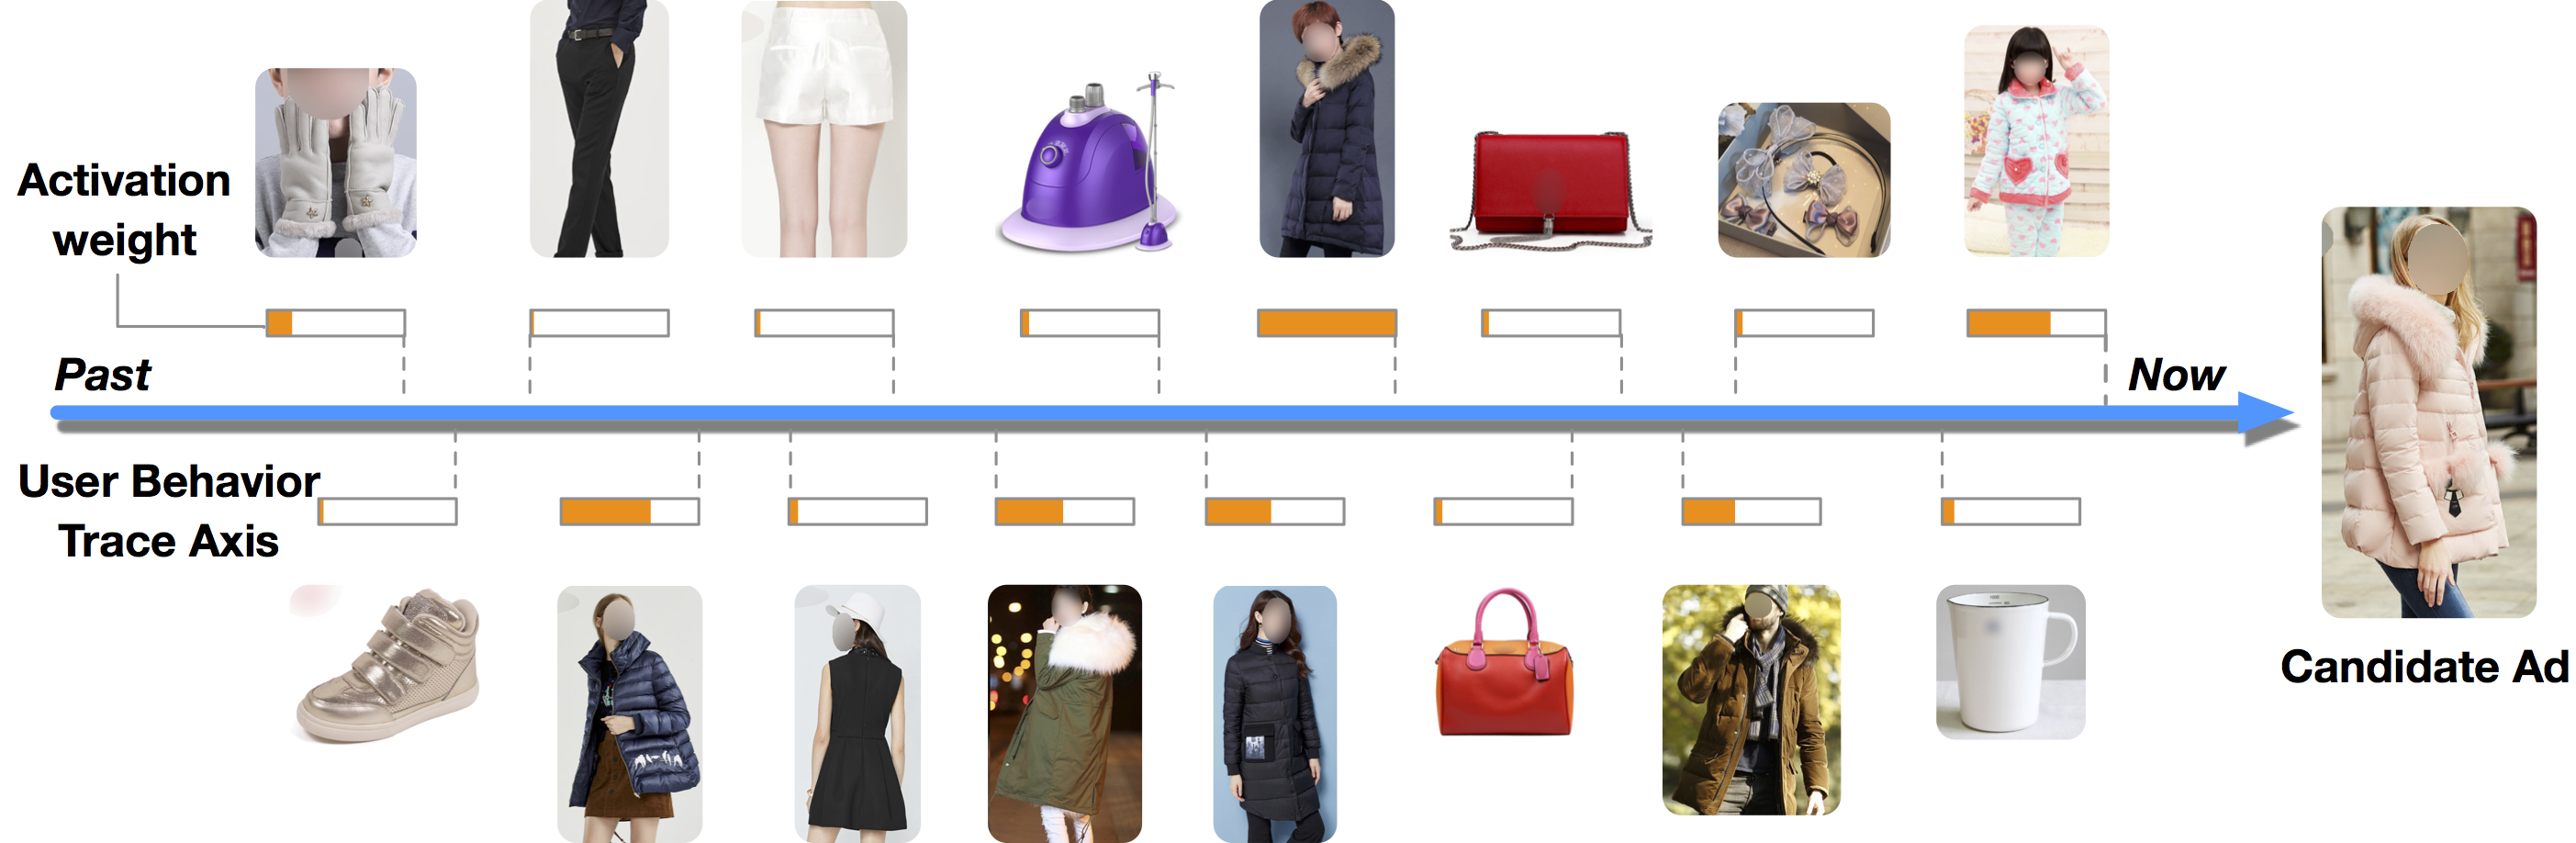
\includegraphics[height=3.5in, width=5in, keepaspectratio]{images/omni/attention_timeline_fix.pdf}
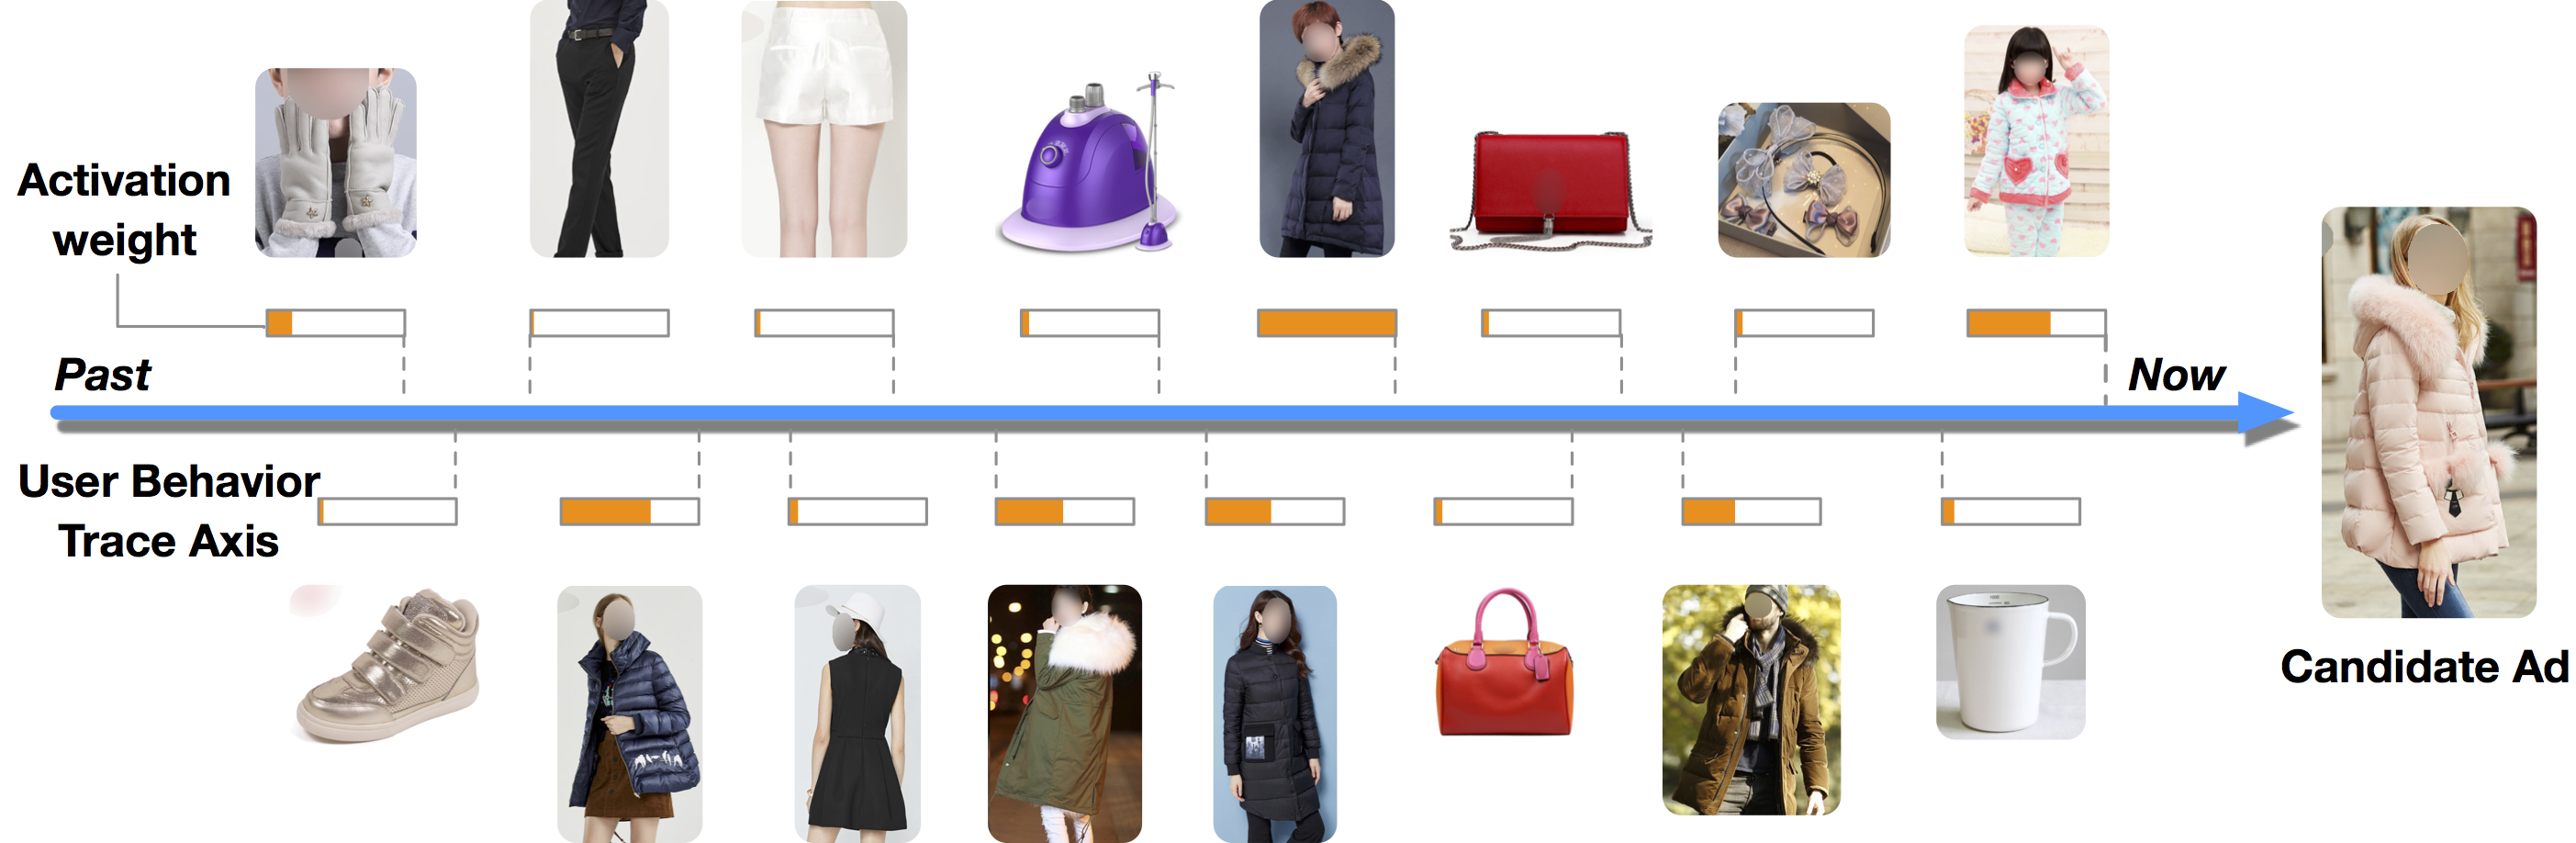
\includegraphics[height=2.5in, width=3.5in, keepaspectratio]{images/omni/attention_timeline_fix.png}
\caption{DIN 中自适应激活示意图。与候选广告高度相关的行为获得较高激活权重。}
\label{fig:att_case}
%\end{figure*}
\end{figure}


随后，我们可视化学习到的 embedding 向量。
以前文提到的年轻母亲为例，我们随机选择 9 个类别，如连衣裙、运动鞋、箱包等，并为每个类别选择 100 个商品作为她的候选广告。
图 \ref{fig:TDdiagram} 展示了 DIN 学习到的商品 embedding 向量的 t-SNE\cite{tsne} 可视化，其中形状相同的点对应同一类别。
可以看到，同一类别的商品几乎属于同一个簇，这清楚展示了 DIN embedding 的聚类性质。
此外，我们按预测值对表示候选广告的点着色。图 \ref{fig:TDdiagram} 也可看作这位母亲在 embedding 空间中对潜在候选项的兴趣密度分布热力图。它表明 DIN 能够在候选项的 embedding 空间中为某个用户形成多峰兴趣密度分布，从而捕获其多样化兴趣。




\begin{figure}[!t]
%\setlength{\belowcaptionskip}{-0.5cm}
\centering
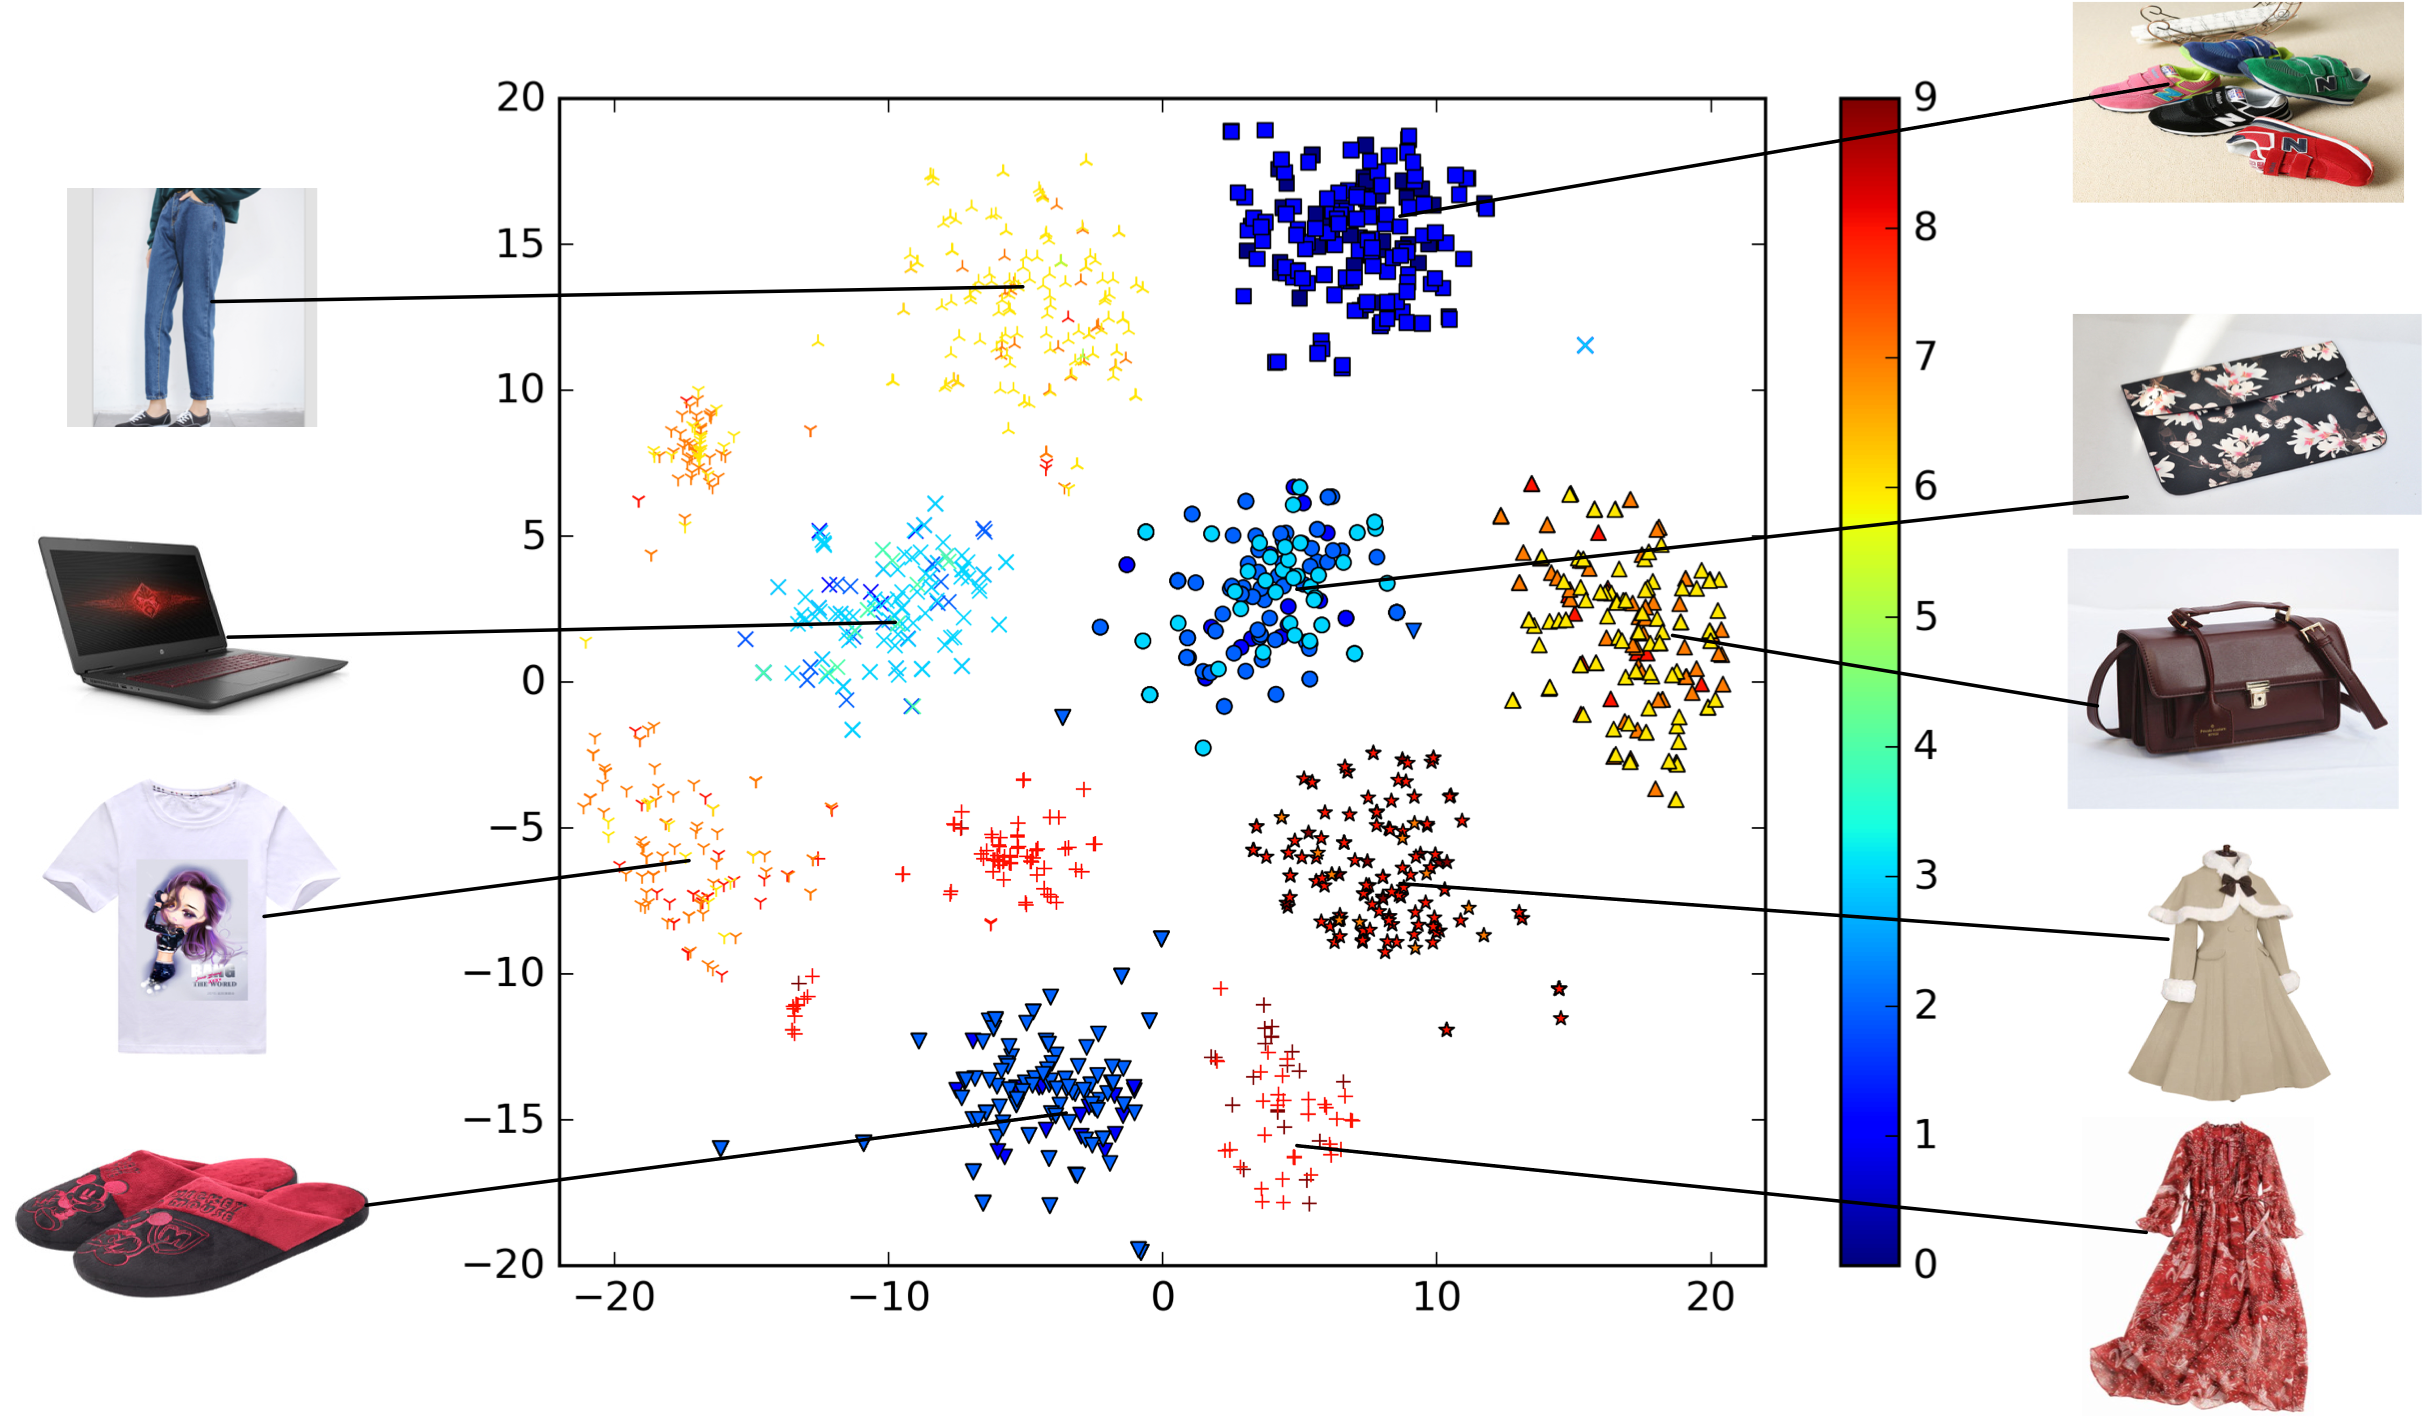
\includegraphics[height=2.5in, width=3.5in, keepaspectratio]{images/omni/TDdiagram.png}
\caption{DIN 中商品 embedding 的可视化。点的形状表示商品类别，点的颜色对应 CTR 预测值。}
\label{fig:TDdiagram}
\end{figure}



%Besides, we color the points that represent candidate ads by the prediction value. 
%Hot(red) points get higher CTR than cold(blue) ones.
%The red points appear in more than one clusters.
%Different categories of goods appearing the her historical behaviors are colored hot(red), which get higher CTR than those random candidates with cold(blue) color.  
%This demonstrates that DIN is able to capture diverse interests of a certain user, by forming a multimodal probability distribution of user interests in the embedding space.

\section{结论}
本文聚焦于电商行业展示广告场景中的 CTR 预测建模任务，该场景具有丰富的用户行为数据。
在传统深度 CTR 模型中使用定长表征，会成为捕获用户兴趣多样性的瓶颈。
为了提升模型表达能力，我们设计了一种名为 DIN 的新方法，用于激活相关用户行为，并获得随广告不同而变化的用户兴趣自适应表征向量。
%soft-searching for a part of user's behaviors to represent user's activated interests with a vector, which varies with candidate ads.\par
%With exploiting these characteristic sufficiently, we design a novel model named DIN.
%Besides, we propose a mini-batch aware regularization technique which can help reducing overfitting greatly in our scenario. What's more, we design a mini-batch aware activation function to accelerate convergence of our model. These approaches could be generalized to other industrial deep learning tasks.
此外，本文引入了两项新技术，以帮助训练工业级深度网络，并进一步提升 DIN 的性能。它们可以容易地推广到其他工业深度学习任务。
DIN 现已部署于阿里巴巴在线展示广告系统。
%DIN now has been deployed in the productive display advertising system in Alibaba and contributes up to 10.0\% CTR promotion compared with BaseModel, our last productive version, which is a significant improvement to the business.
%Experiments show that DIN brings more interpretability and achieves better GAUC performance compared with popular Embedding\&MLP model.
%=======
%We reveal and summarize the two key characteristics of data: diversity and local activation. With exploiting these characteristics sufficiently, we design a novel model named DIN.
%Experiments show that DIN brings more interpretability and achieves better GAUC performance compared with popular Embedding\&MLP model.
%Besides, we propose a mini-batch aware regularization technique which can help reducing overfitting greatly in our scenario. What's more, we design a new activation function based on data to accelerate convergence of our model. We suppose these approaches could be instructive to other industrial deep learning tasks.\par
%>>>>>>> 802ff3c7671abeecb6185253b8389137e6009ec9
%Different from the fields of image recognition and natural language process with mature and state-of-the-art deep network structures, applications with rich internet-scale user behavior data still face a lot of challenges. These applications are worth making more efforts to study and improve. We will continue to focus on this direction.

%\section{Future work}
%With better understanding the diversity and local activation effects of user's interests, DIN captures users' interests effectively. It's notable that the users' behavior data is sequential, which may reflect user intentions further. But user's behavior sequence contains concurrent multiple varying interests and rapid jumping over these diverse interests, which make the sequence seems noisy and disordering. Our proposed attention-like activation network can filter out the relevant single-interest sub-sequence, making the sequence analysis easier. However, in e-commerce scenario, special characteristics of the behavior sequence need to be carefully studied, e.g., the first-activation, termination (like due to one purchasing behavior), possible reactivation (like periodic repeat purchase) of one sequential interest, which are all mixed in the user's concurrent multiple different interest sequences. One future direction is to design more delicate structure to capture interests from sequential historical behavior better.\par

%the sequential characteristic of user historical behavior is weak and noisy, which may be affected by both users' interests and system factors. So, in future, we will focus on
%What's more, many methods on task of CTR prediction in a real online system do experiment on their own industry dataset, which makes it difficult to compare fairly. We plan to publish the dataset after desensitizing from our advertising display system. We wish it could help the standardization of the experiment later.


\bibliographystyle{ACM-Reference-Format}
\bibliography{DIN} 
\end{document}
